\chapter{Wyniki badań\@}
\label{ch:wyniki}

W niniejszym rozdziale zostaną przedstawione rezultaty eksperymentów dotyczących wykorzystania samogłosek /a/, /e/, /i/, /o/ oraz /u/ w procesie automatycznej diagnostyki choroby Parkinsona.
Wcześniej omówione zostały teoretyczne podstawy oraz użyte modele i metody badawcze.
Niniejsza część pracy zawiera wyniki uzyskane po przeprowadzeniu badań obejmujących porównanie różnych modeli opartych na popularnych architekturach sieci neuronowych, mające na celu ocenę ich skuteczności w identyfikacji choroby Parkinsona.
Należy zaznaczyć, że w pracy przedstawiono jedynie najlepsze z uzyskanych wyników.
Tabele~\ref{tab:wyniki-a},~\ref{tab:wyniki-e},~\ref{tab:wyniki-i},~\ref{tab:wyniki-o} oraz~\ref{tab:wyniki-u} przedstawiają średnie z wyników otrzymanych z wykorzystaniem 10-krotnej walidacji krzyżowej.


\section{Samogłoska /a/}
\label{sec:samogloska-a}

Samogłoska /a/ jest wybierana najczęściej jako podstawa analizy w podobnych procesach badawczych.
Ponadto często przy jej wykorzystaniu osiągane są najwyższe wyniki.
Podczas eksperymentów w przypadku samogłoski /a/ najlepszą skuteczność uzyskano wykorzystując architekturę VGG16.
Każda z badanych metryk (dokładność, czułość, precyzja oraz parametr F1) oscylowała w okolicy 75\%.
Kolejne dwie architektury, dla których osiągnięto zadowalające wyniki na poziomie ponad 70\% to ResNet50 i MobileNetV2.
Najgorzej z tym zadaniem, biorąc pod uwagę skuteczność, poradziła sobie architektura Xception.

\begin{table}[ht]
\centering
\caption{Wyniki otrzymane dla samogłoski /a/}
\label{tab:wyniki-a}
\begin{tabular}{|l|c|c|c|c|c|}
\hline
\textbf{Model} &\textbf{VGG16} &\textbf{Resnet50} &\textbf{Xception} &\textbf{InceptionV3} &\textbf{MobileNetV2} \\ \hline
    Accuracy &0.751 &0.724 &0.672 &0.692 &0.714 \\ \hline
    Precision &0.752 &0.703 &0.669 &0.721 &0.712 \\ \hline
    Recall &0.751 &0.713 &0.663 &0.689 &0.709 \\ \hline
    F1-score &0.749 &0.727 &0.675 &0.688 &0.711 \\ \hline
    Loss &0.645 &0.563 &0.611 &0.676 &0.750 \\ \hline
\end{tabular}
\end{table}

Analiza wartości funkcji straty dla różnych modeli wskazuje na zróżnicowaną skuteczność w procesie minimalizacji błędu.
Model ResNet50 osiągnął najniższy wynik straty (0,563), co sugeruje jego lepszą zdolność do generalizacji na dane testowe.
Jednakże, modele VGG16 (0,645) i Xception (0,611) również uzyskały akceptowalne wyniki, podczas gdy model MobileNetV2 (0,750) wypada pod tym względem najsłabiej.
Wszystkie z przedstawionych rozwiązań mogą wymagać dalszej optymalizacji lub dostrojenia parametrów w celu poprawy skuteczności.
Szczegółowe wartości zostały zawarte w tabeli~\ref{tab:wyniki-a}.

\begin{figure}[ht]
    \centering
    \begin{subfigure}{0.49\textwidth}
        \centering
        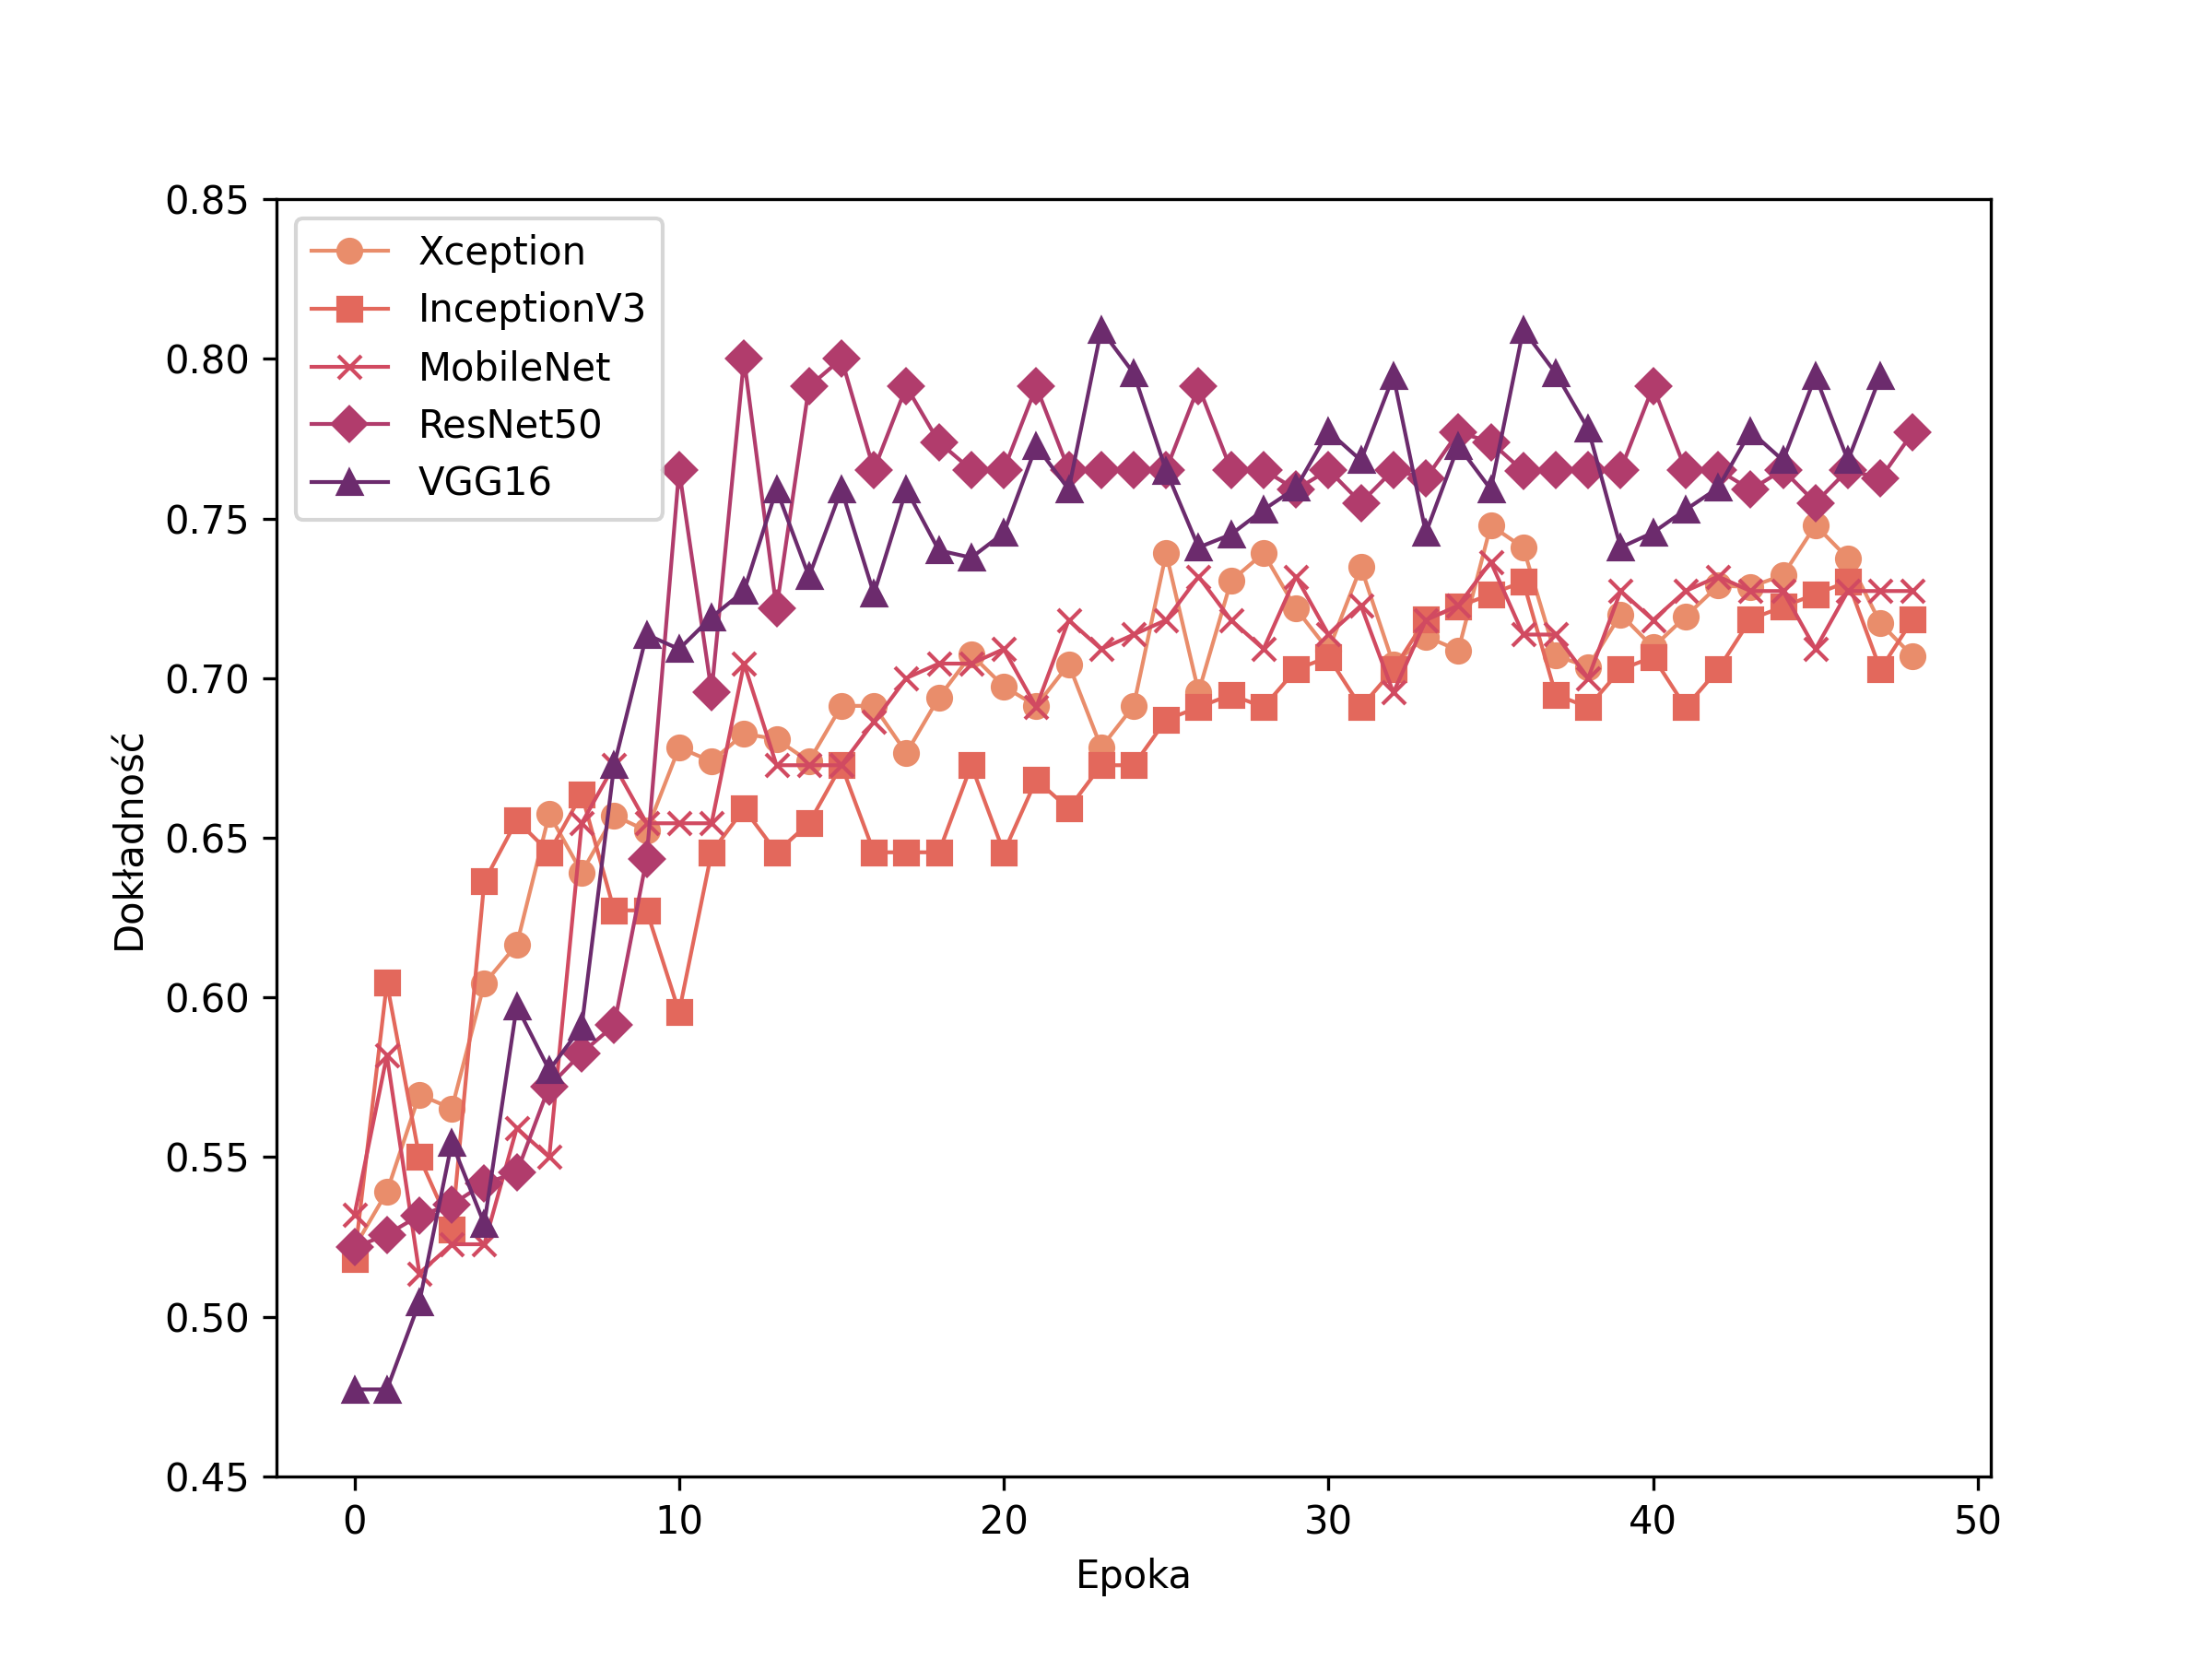
\includegraphics[width=\textwidth]{./img/results/a_acc}
        \caption{Krzywe dokładności na zbiorze walidacyjnym\@}
        \label{fig:a_acc}
    \end{subfigure}
    \begin{subfigure}{0.49\textwidth}
        \centering
        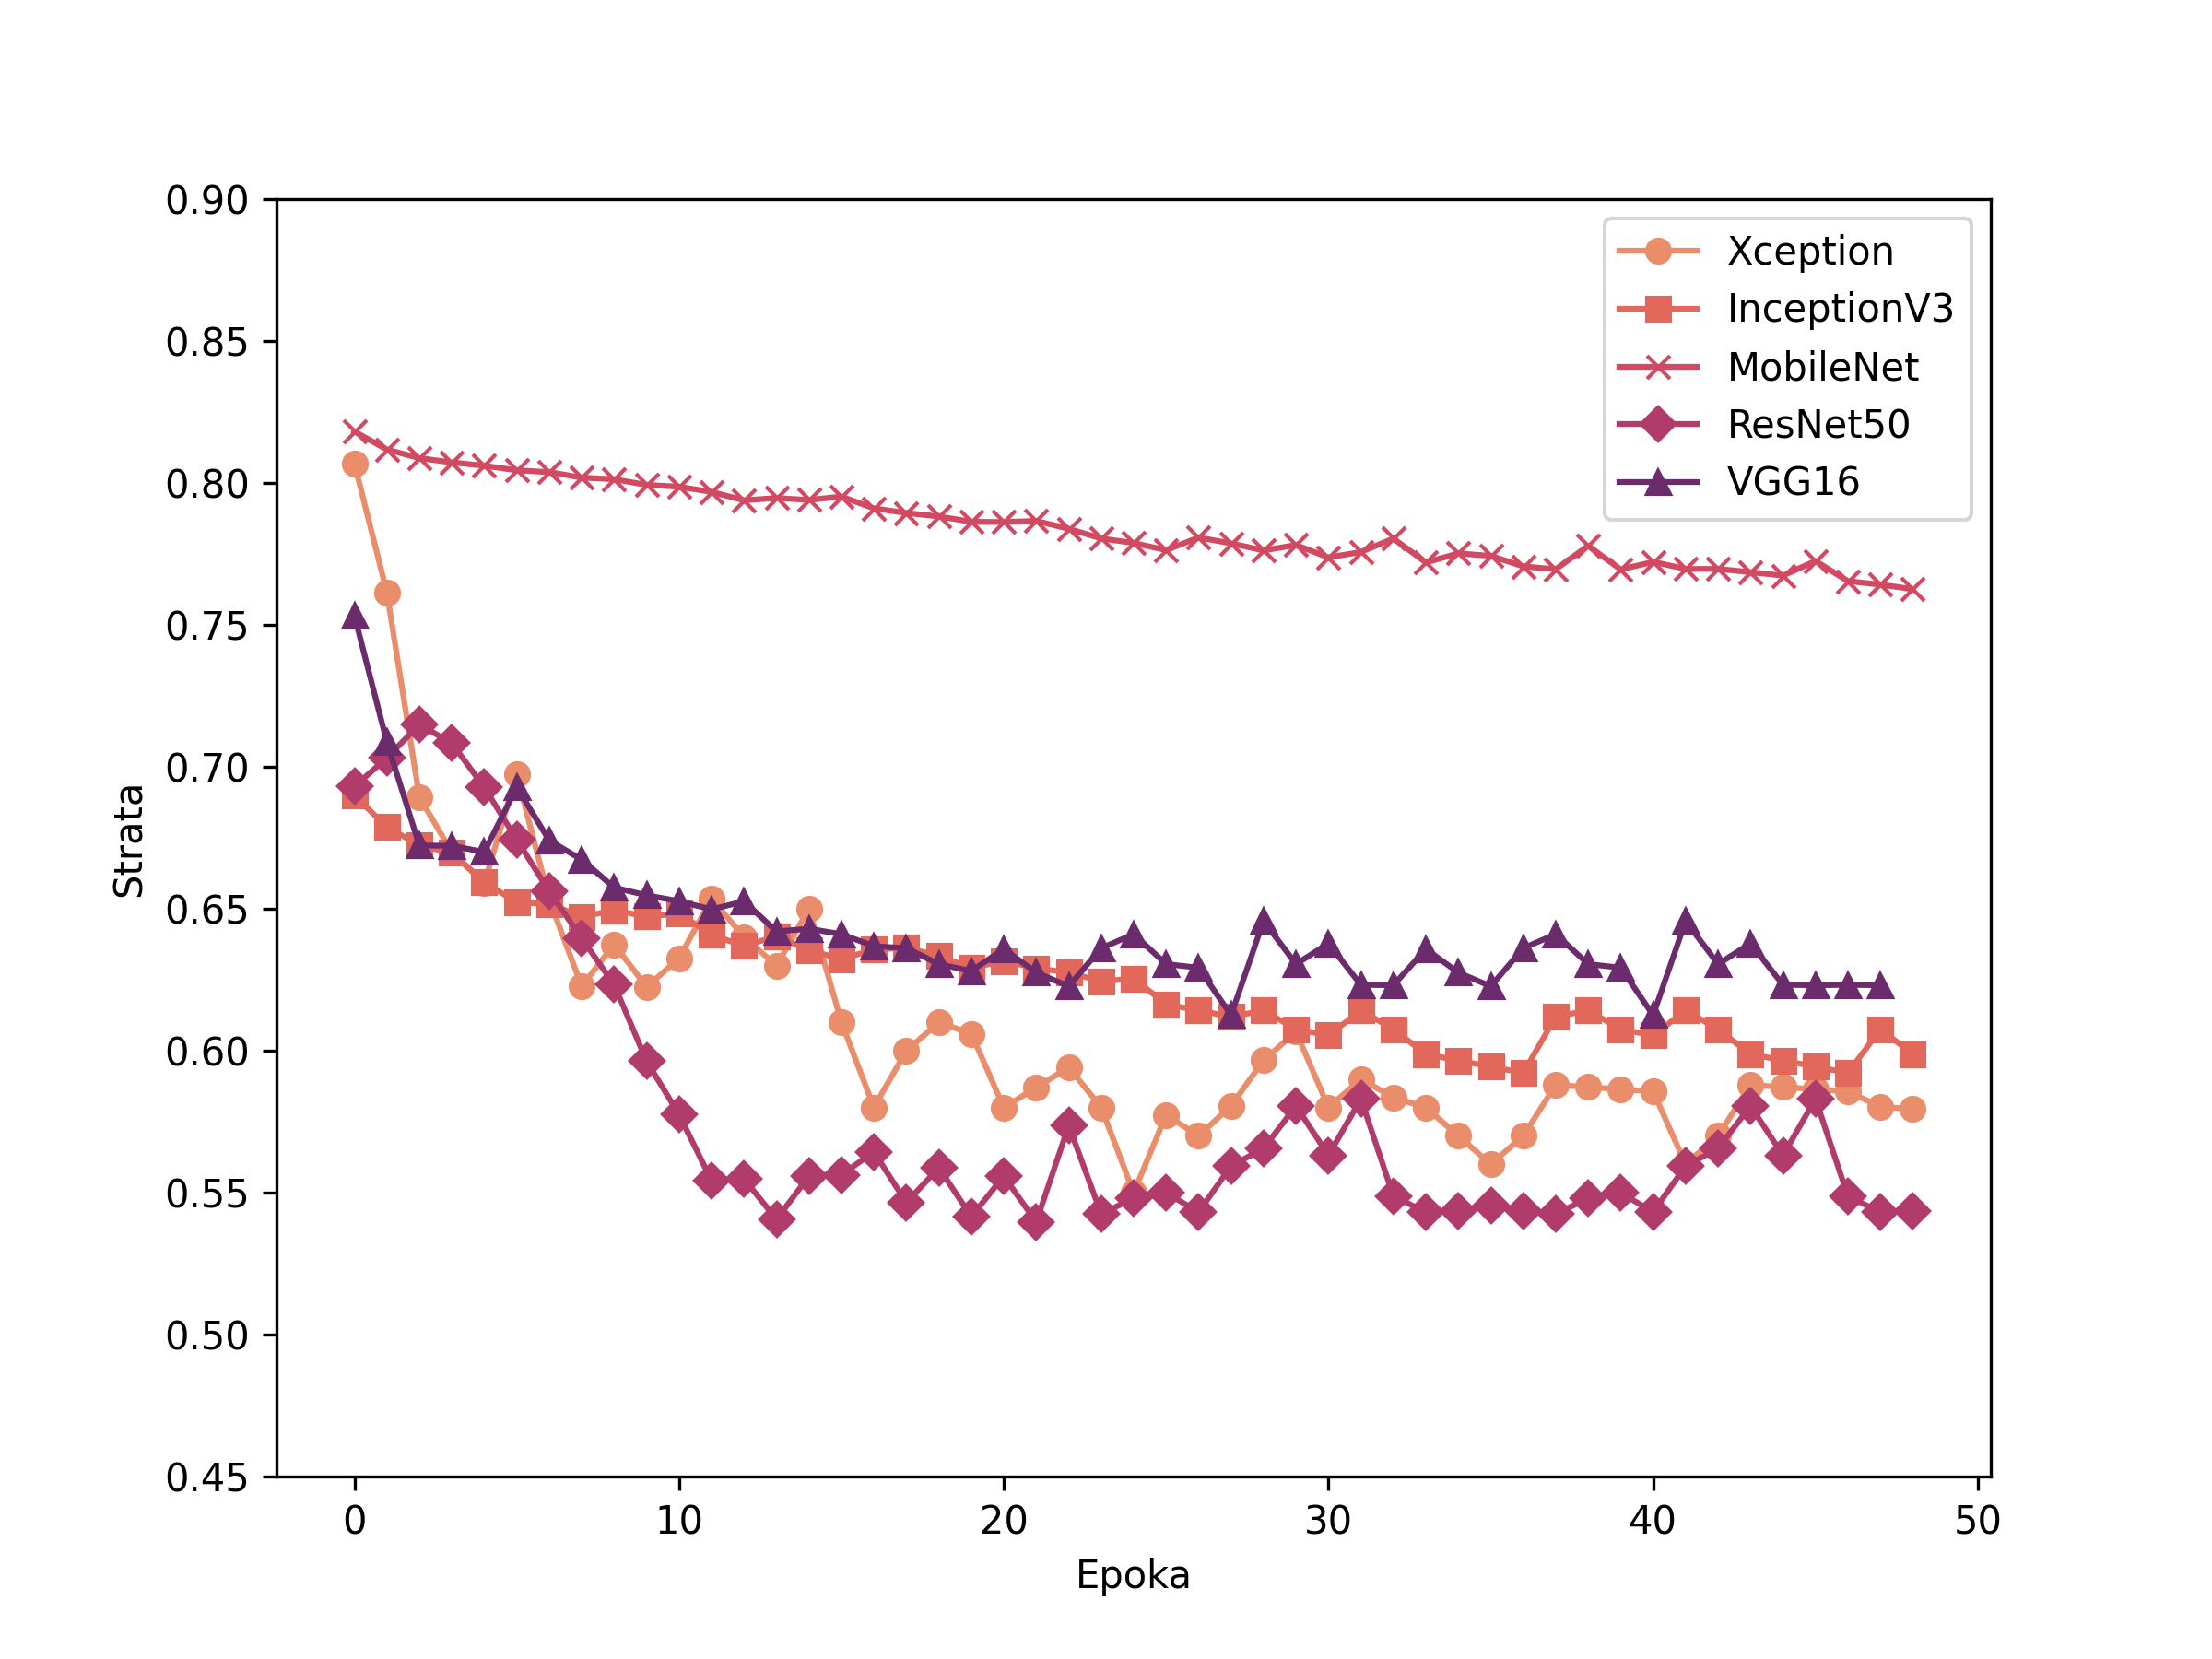
\includegraphics[width=\textwidth]{./img/results/a_loss}
        \caption{Krzywe funkcji straty na zbiorze walidacyjnym\@}
        \label{fig:a_loss}
    \end{subfigure}

    \caption{Porównanie krzywych uczenia dla różnych klasyfikatorów na zbiorze walidacyjnym (samogłoska /a/)}
    \label{fig:a_results}
\end{figure}

Analizując proces uczenia na zbiorze walidacyjnym (Rys.~\ref{fig:a_results}),  można stwierdzić, że przebiegał on podobnie w większości przypadków.
Wartości osiągnięte na tym zbiorze były zbliżone do wyników uzyskanych na zbiorze testowym, co wskazuje na zdolność modeli do generalizacji.
Wykresy reprezentujące różne klasyfikatory wykazują podobne tendencje, jednak krzywa funkcji straty w przypadku modelu MobileNetV2 wykazuje pewne odchylenia od pozostałych.
To może sugerować, że MobileNetV2 reaguje inaczej na dane walidacyjne, co może mieć wpływ na jego ogólną skuteczność.
Na podstawie przedstawionych wyników można wyróżnić model VGG16 jako potencjalnie najlepszy w przypadku diagnostyki choroby Parkinsona na podstawie samogłoski /a/.
Dobrym wyborem byłby również niewiele odbiegający ResNet50, wykazujący się niższą wartością funkcji straty.
%---------------------------------------------------------------------------

\section{Samogłoska /e/}
\label{sec:samogloska-e}

W przypadku samogłoski /e/ otrzymano wyniki nieco gorsze, ale zbliżone do tych uzyskanych w przypadku samogłoski /a/.
Tym razem również architektury VGG16 (73\%) i MobileNetV2 (70\%) osiągnęły najwyższą skuteczność, co wskazuje na ich potencjał w tym zadaniu klasyfikacyjnym.
Wartości funkcji straty wahają się od 0,582 (dla VGG16) do 0,659 (dla ResNet50).
Jest to istotna informacja, ponieważ niższa wartość straty może sugerować lepszą zdolność modelu do dokładnej klasyfikacji.
Warto zwrócić uwagę, że architektura ResNet50 (62\%) uzyskała najniższą dokładność w tym przypadku, mimo wysokich wyników dla samogłoski /a/.
Raport przedstawiony został w tabeli~\ref{tab:wyniki-e}.

\begin{table}[ht]
\centering
\caption{Wyniki otrzymane dla samogłoski /e/}
\label{tab:wyniki-e}
\begin{tabular}{|l|c|c|c|c|c|}
\hline
\textbf{Model} &\textbf{VGG16} &\textbf{Resnet50} &\textbf{Xception} &\textbf{InceptionV3} &\textbf{MobileNetV2} \\ \hline
    Accuracy &0.733 &0.621 &0.653 &0.644 &0.700 \\ \hline
    Precision &0.729 &0.625 &0.640 &0.641 &0.721 \\ \hline
    Recall &0.733 &0.620 &0.633 &0.638 &0.689 \\ \hline
    F1-score &0.735 &0.643 &0.649 &0.640 &0.692 \\ \hline
    Loss &0.582 &0.659 &0.632 &0.634 &0.601 \\ \hline
\end{tabular}
\end{table}


\begin{figure}[ht]
    \centering
    \begin{subfigure}{0.49\textwidth}
        \centering
        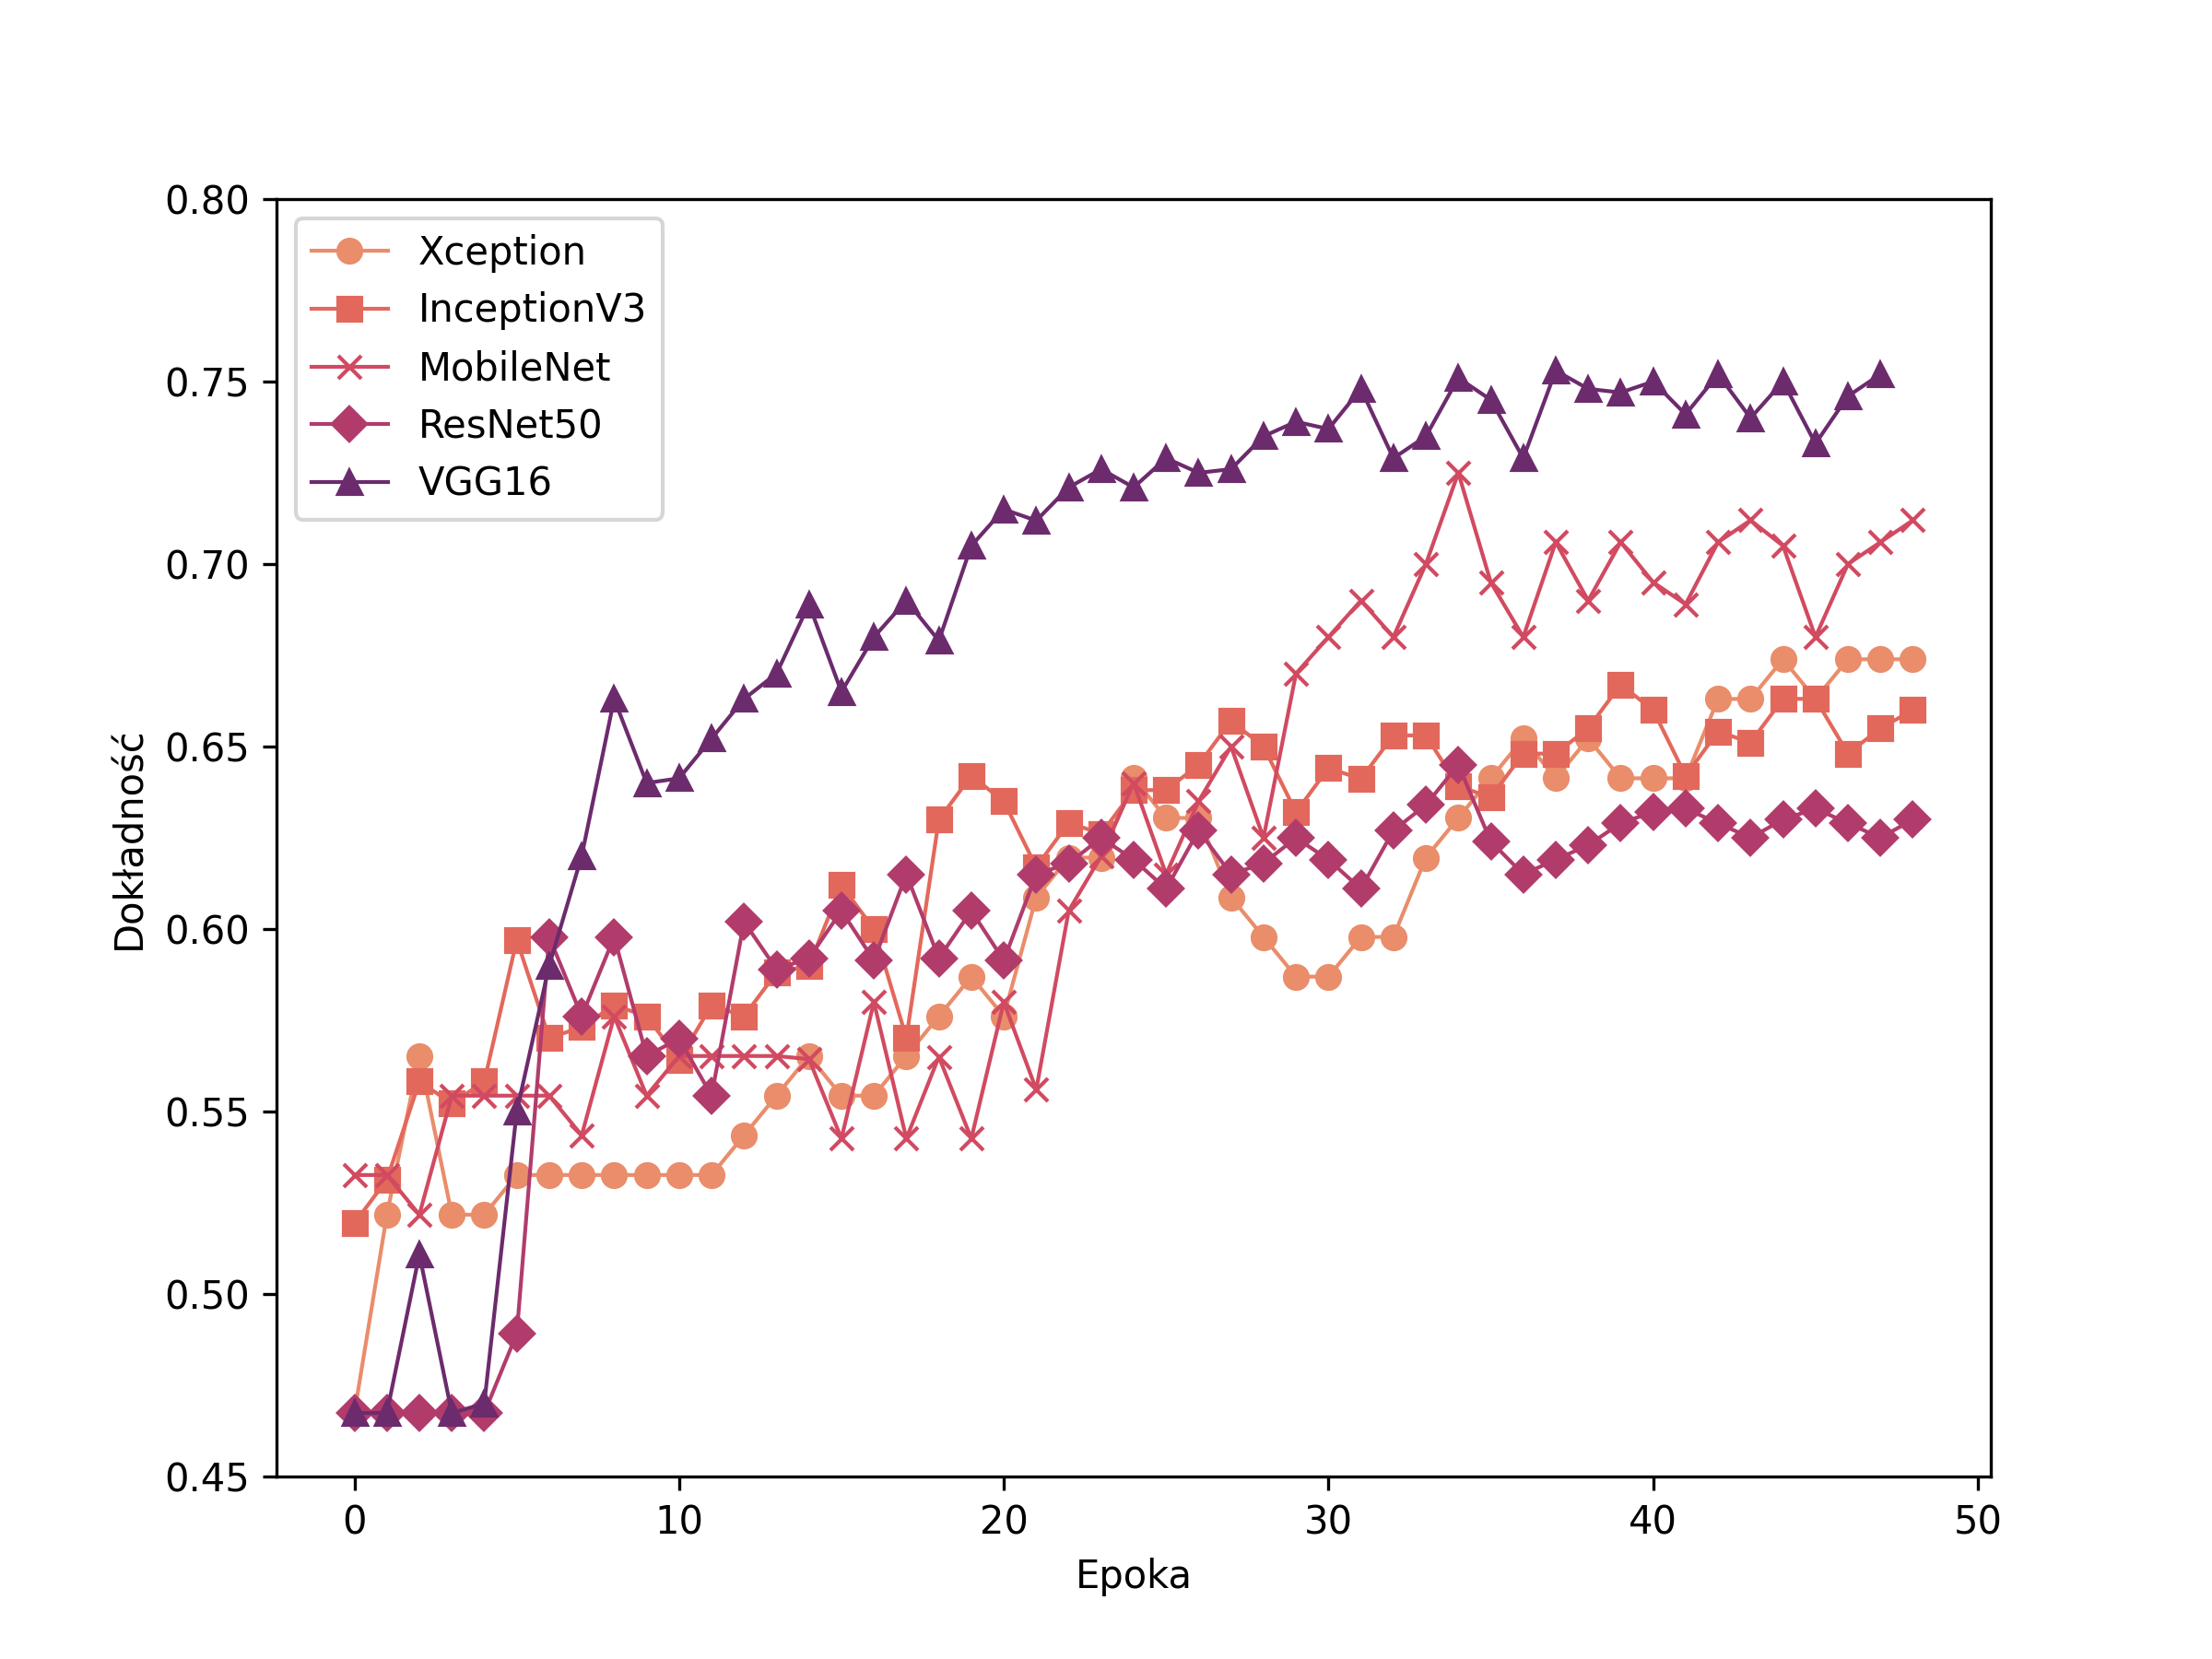
\includegraphics[width=\textwidth]{./img/results/e_acc}
        \caption{Krzywe dokładności na zbiorze walidacyjnym\@}
        \label{fig:e_acc}
    \end{subfigure}
    \begin{subfigure}{0.49\textwidth}
        \centering
        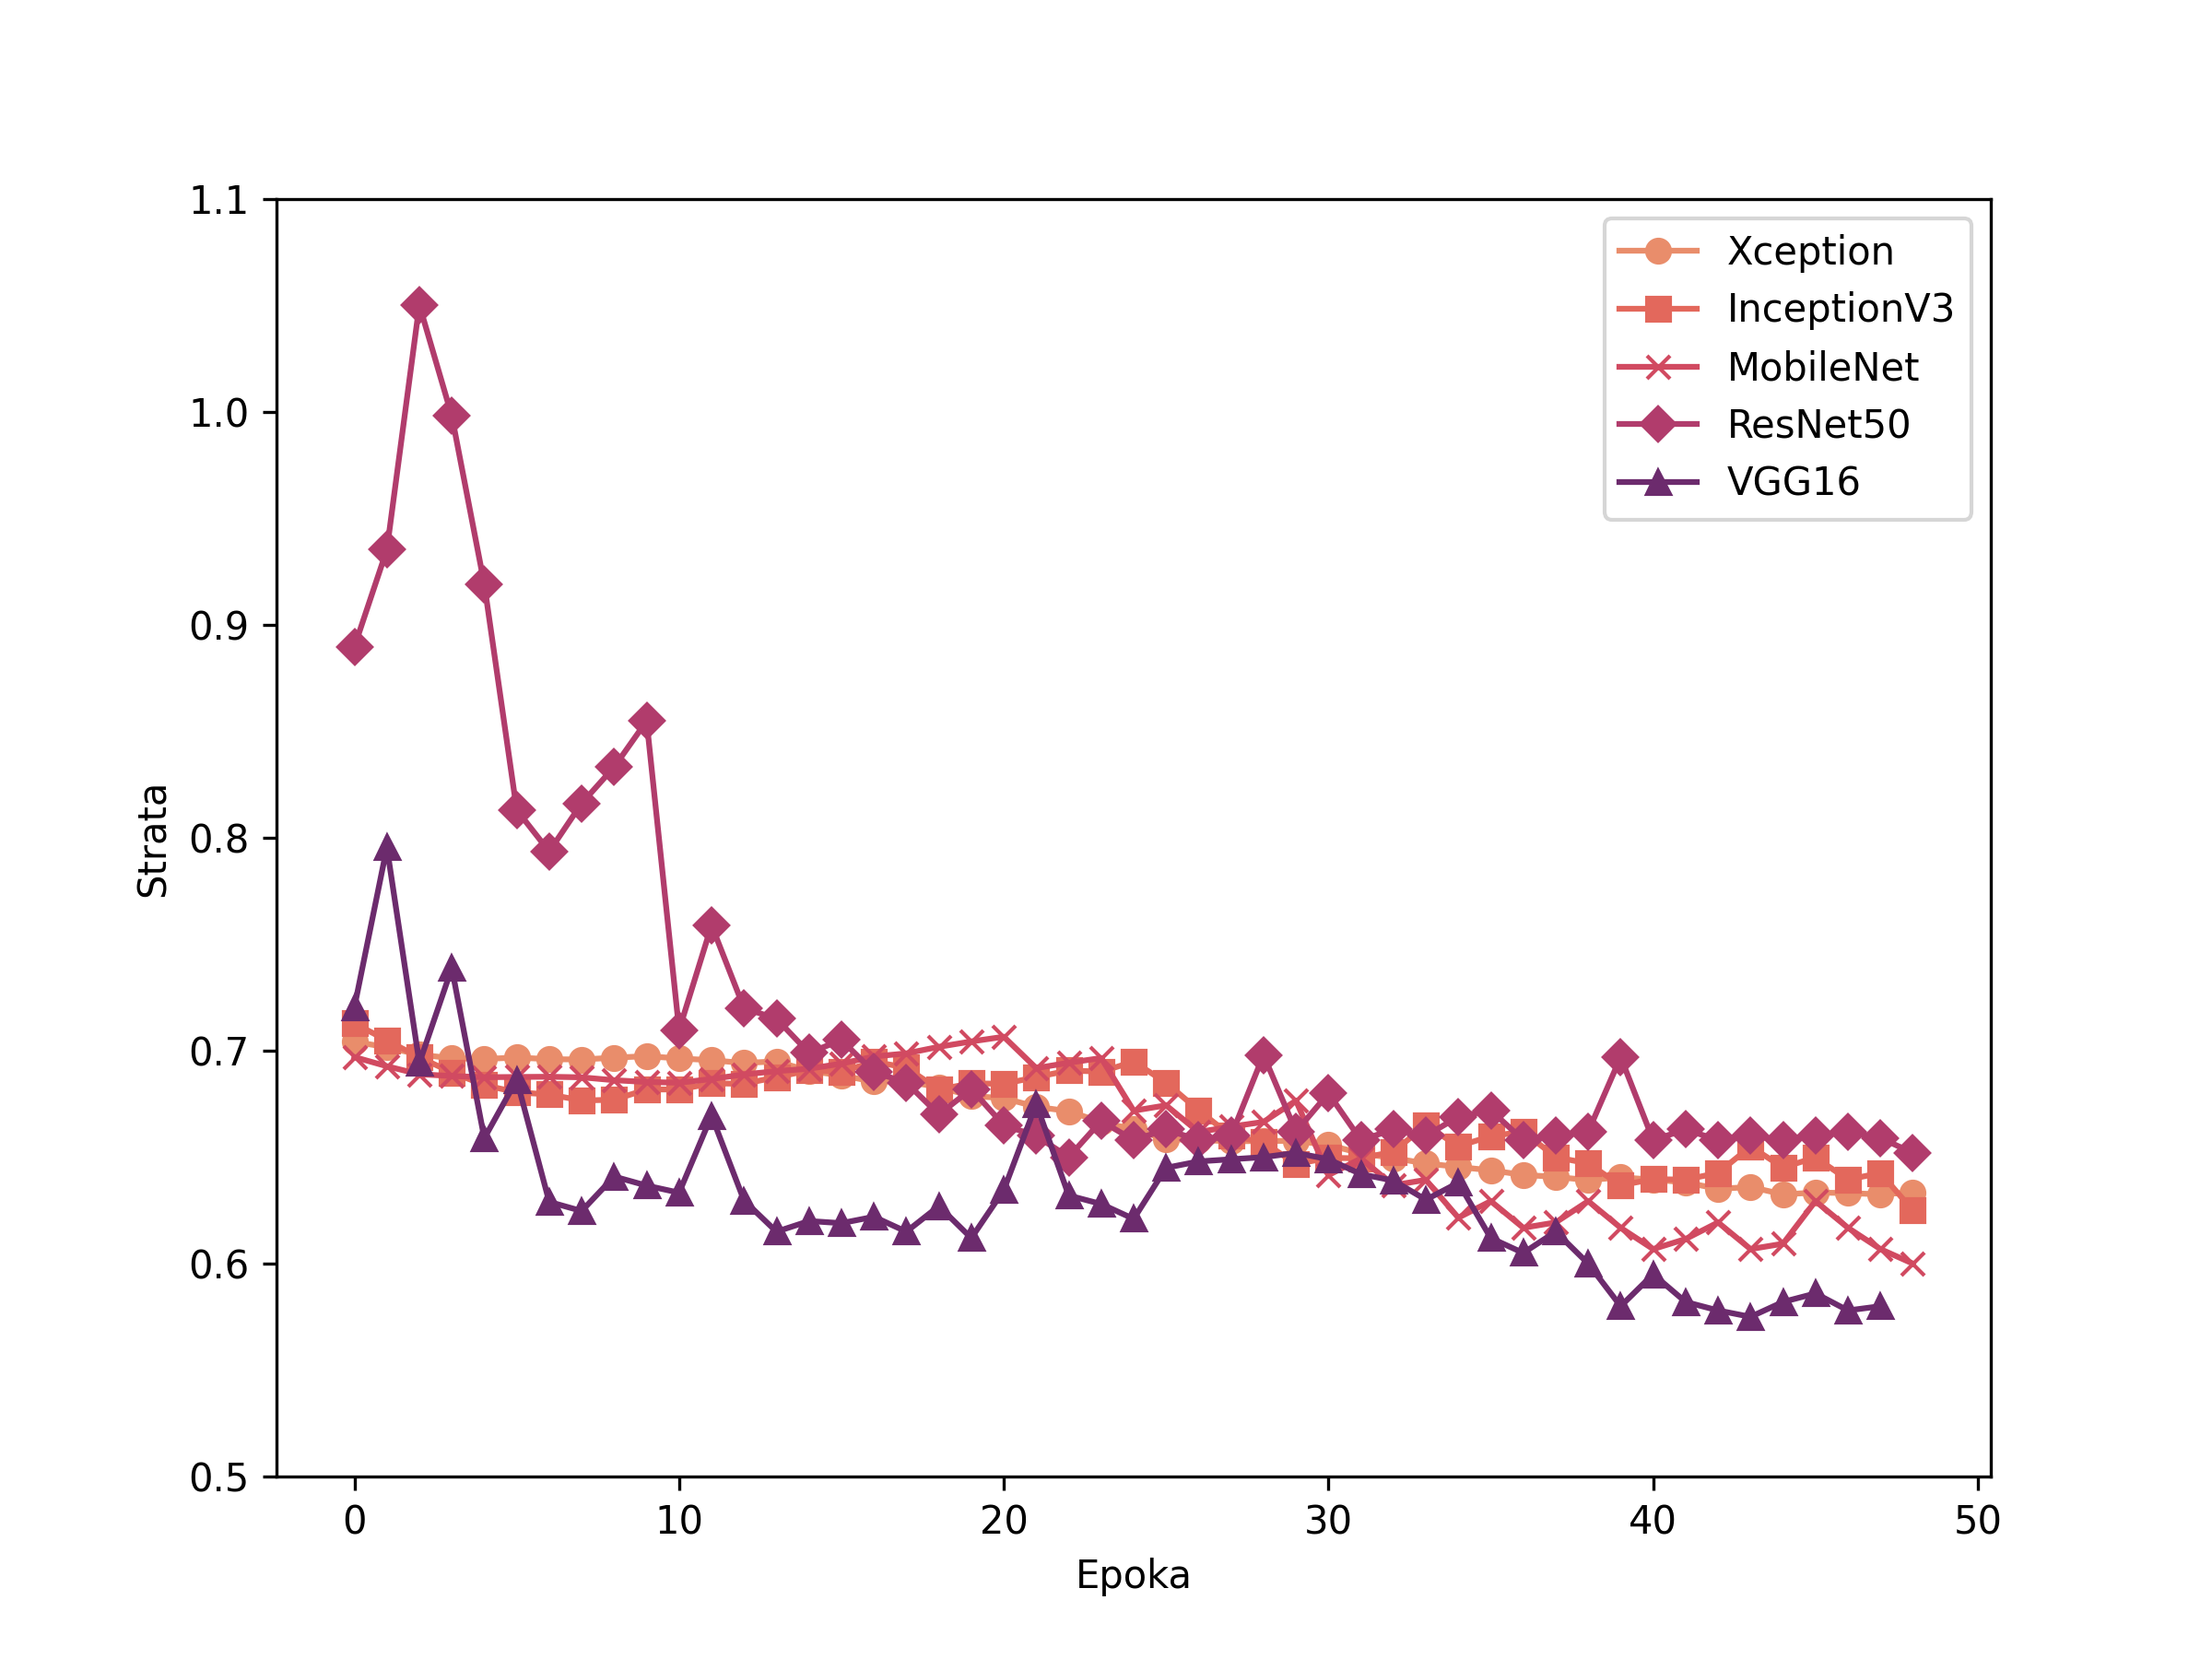
\includegraphics[width=\textwidth]{./img/results/e_loss}
        \caption{Krzywe funkcji straty na zbiorze walidacyjnym\@}
        \label{fig:e_loss}
    \end{subfigure}

    \caption{Porównanie krzywych uczenia dla różnych klasyfikatorów na zbiorze walidacyjnym (samogłoska /e/)}
    \label{fig:e_results}
\end{figure}

Jeśli chodzi o zachowanie modelu w trakcie procesu uczenia, można zauważyć, że było ono podobne we wszystkich przypadkach, co zostało zobrazowane na Rys.~\ref{fig:e_results}.
Modele osiągały względną stabilność w różnych momentach procesu uczenia i różniły się tempem dostosowywania się do danych treningowych oraz początkowymi wartościami funkcji straty w kilku pierwszych epokach.
Jednak na końcu procesu uczenia wartości te były zbliżone do siebie i odzwierciedlały te uzyskane na zbiorze testowym.
Nie zaobserwowano wyraźnego przeuczenia (ang. \emph{overfittingu}) modeli, co jest pozytywnym wynikiem eksperymentu.
Na tle pozostałych ponownie najlepiej sprawdził się model VGG16.
%---------------------------------------------------------------------------

\section{Samogłoska /i/}
\label{sec:samogloska-i}

W przypadku samogłoski /i/ można zauważyć, że wyniki uległy pogorszeniu w porównaniu do samogłoski /a/ oraz /e/.
Najlepsze rezultaty uzyskano przy wykorzystaniu architektur MobileNetV2 i VGG16, gdzie dokładność wyniosła około 63\%.
Warto zaznaczyć, że jest to znacznie niższy poziom dokładności w porównaniu do wyników uzyskanych dla samogłoski /a/.
Szczególnie niski wynik obserwuje się ponownie dla modelu ResNet50, który osiągnął tylko około 59\% dokładności.

Wartości funkcji straty są natomiast bardzo wysokie, w zakresie od 0,656 dla MobileNetV2 do 0,775 dla VGG16.
To może sugerować, że informacja diagnostyczna zawarta w samogłosce /i/ jest trudniej dostępna w porównaniu do innych samogłosek, co wpływa na wyższe wartości straty i niższą dokładność.
Możliwe jest, że inne samogłoski mogą dostarczać bardziej wyraźnych i łatwiejszych do interpretacji sygnałów diagnostycznych.
Szczegółowe wartości przedstawia tabela~\ref{tab:wyniki-i}.

\begin{table}[ht]
\centering
\caption{Wyniki otrzymane dla samogłoski /i/}
\label{tab:wyniki-i}
\begin{tabular}{|l|c|c|c|c|c|}
\hline
\textbf{Model} &\textbf{VGG16} &\textbf{Resnet50} &\textbf{Xception} &\textbf{InceptionV3} &\textbf{MobileNetV2} \\ \hline
    Accuracy &0.627 &0.586 &0.641 &0.605 &0.634 \\ \hline
    Precision &0.642 &0.589 &0.638 &0.598 &0.672 \\ \hline
    Recall &0.616 &0.584 &0.642 &0.595  &0.623 \\ \hline
    F1-score &0.605 &0.572 &0.643 &0.597 &0.614 \\ \hline
    Loss &0.775 &0.699 &0.705 &0.686 &0.656 \\ \hline
\end{tabular}
\end{table}

\begin{figure}[ht]
    \centering
    \begin{subfigure}{0.49\textwidth}
        \centering
        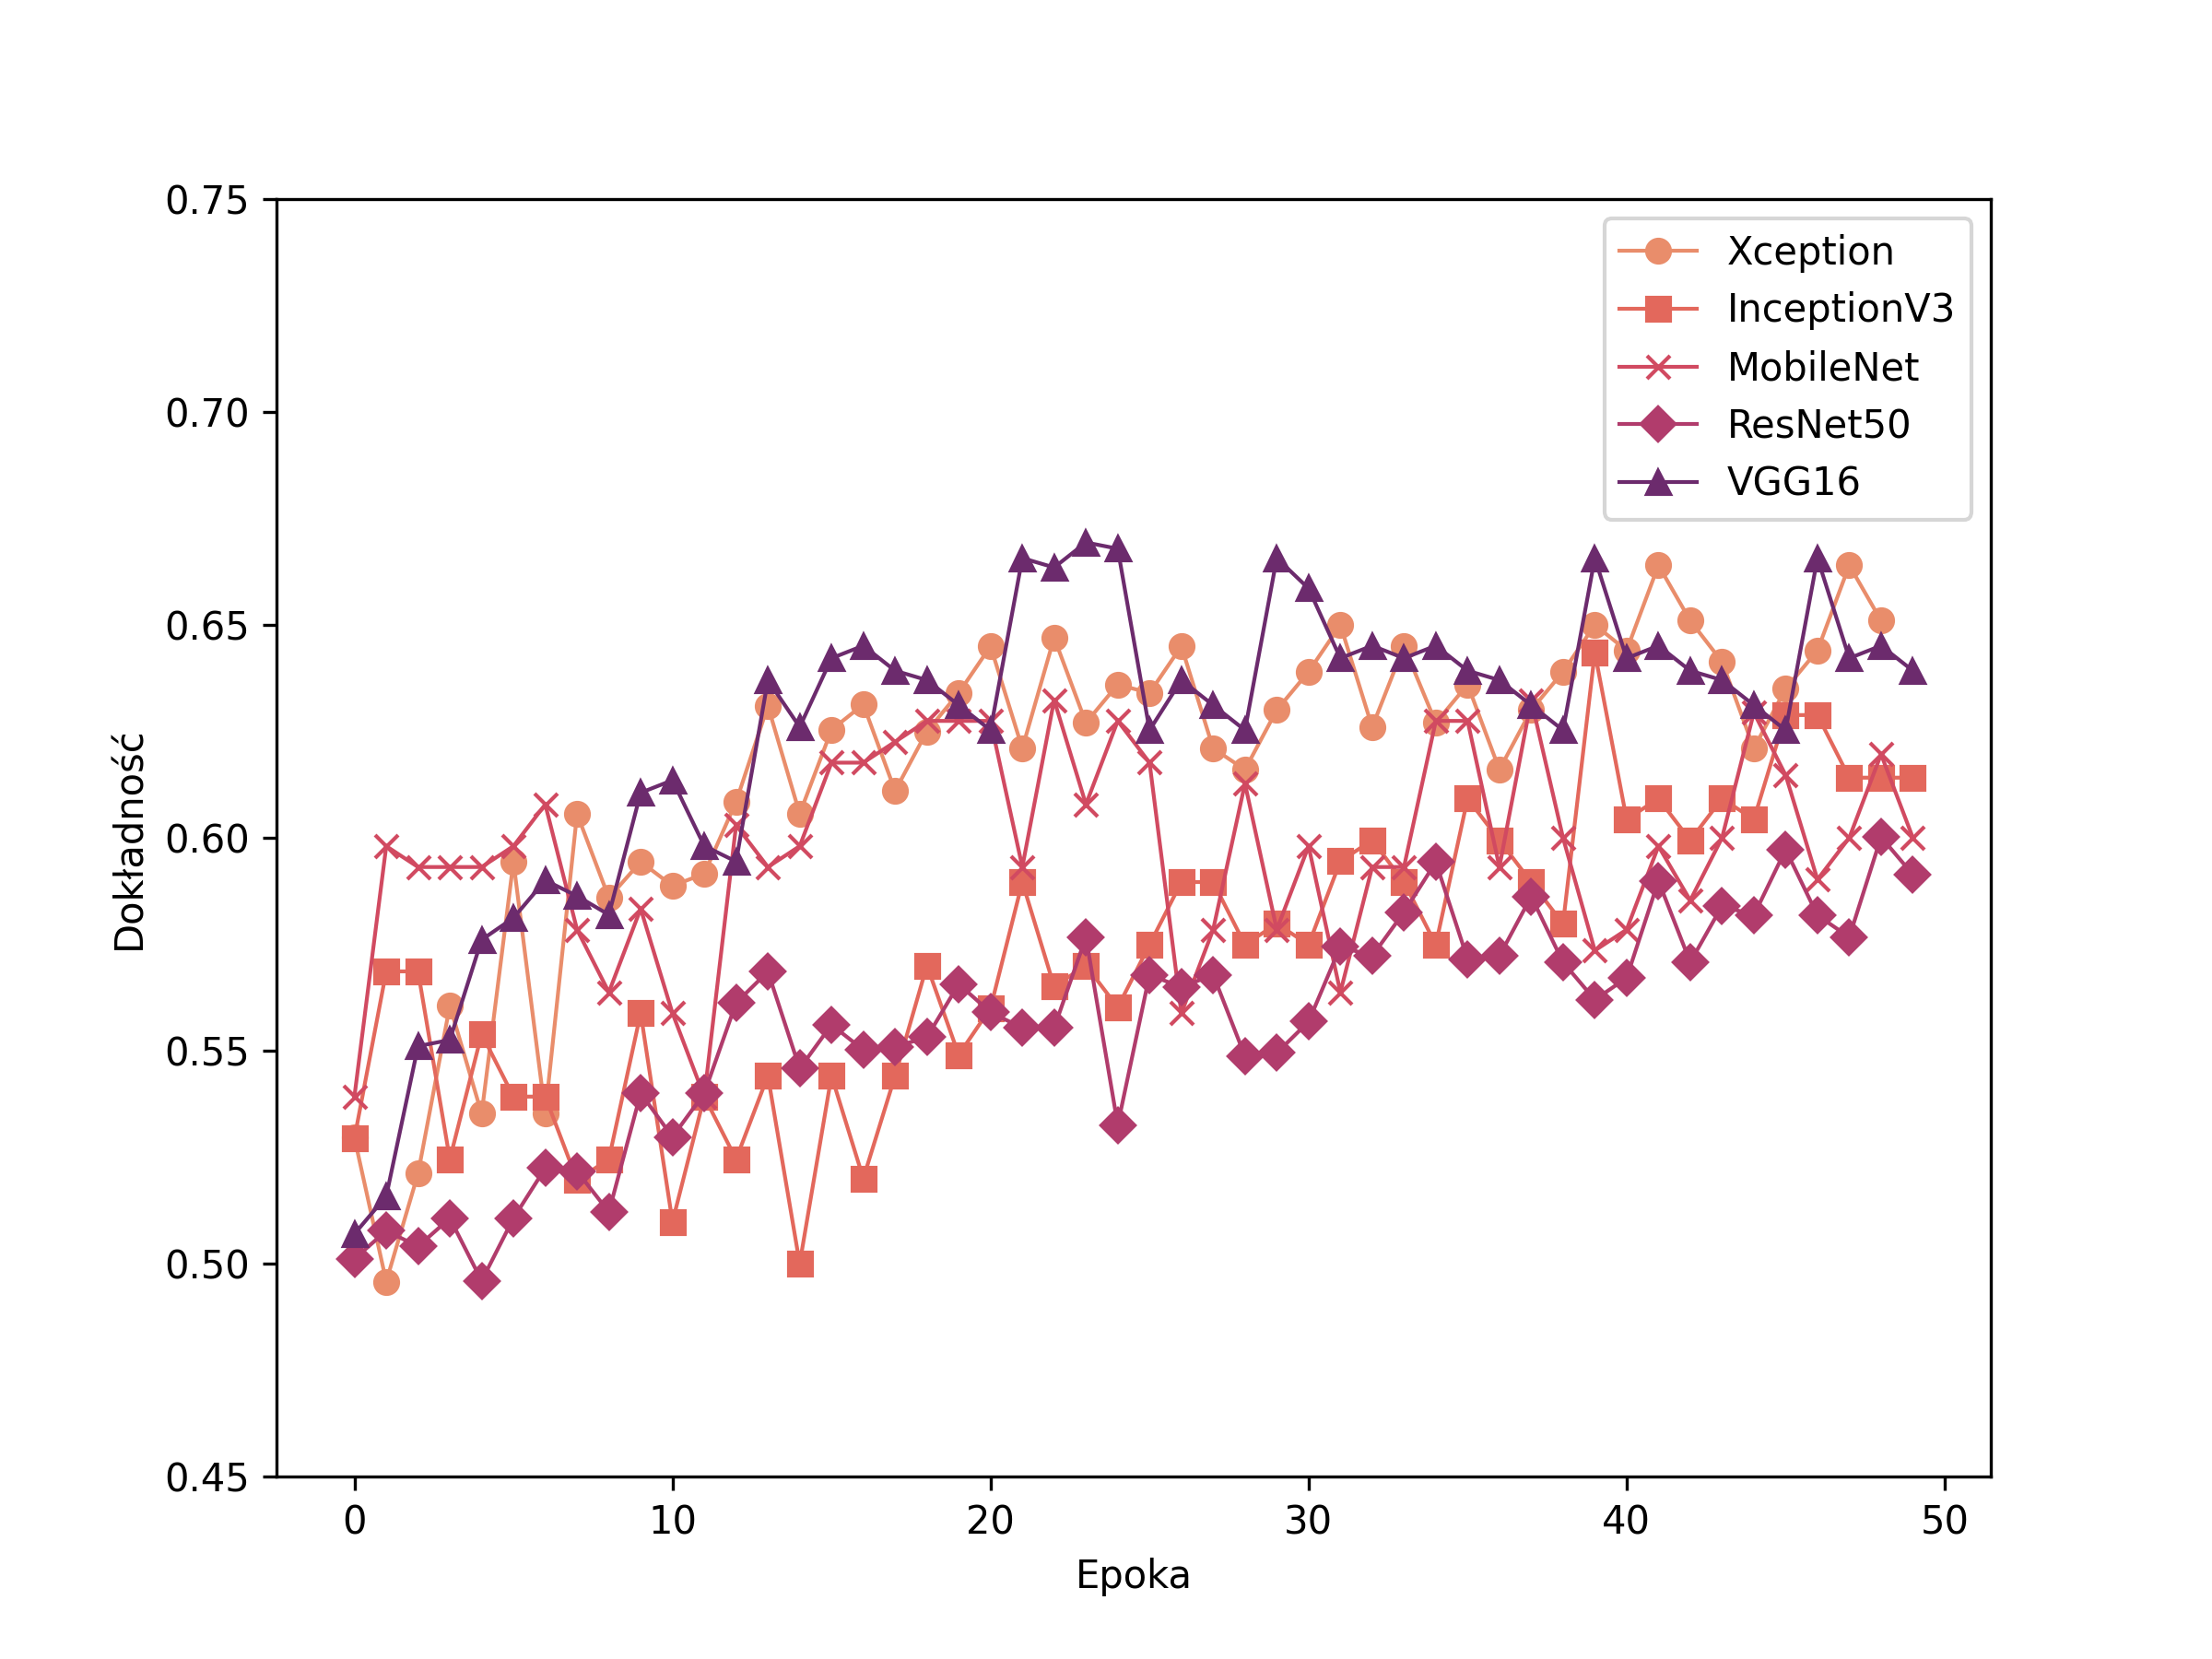
\includegraphics[width=\textwidth]{./img/results/i_acc}
        \caption{Krzywe dokładności na zbiorze walidacyjnym\@}
        \label{fig:i_acc}
    \end{subfigure}
    \begin{subfigure}{0.49\textwidth}
        \centering
        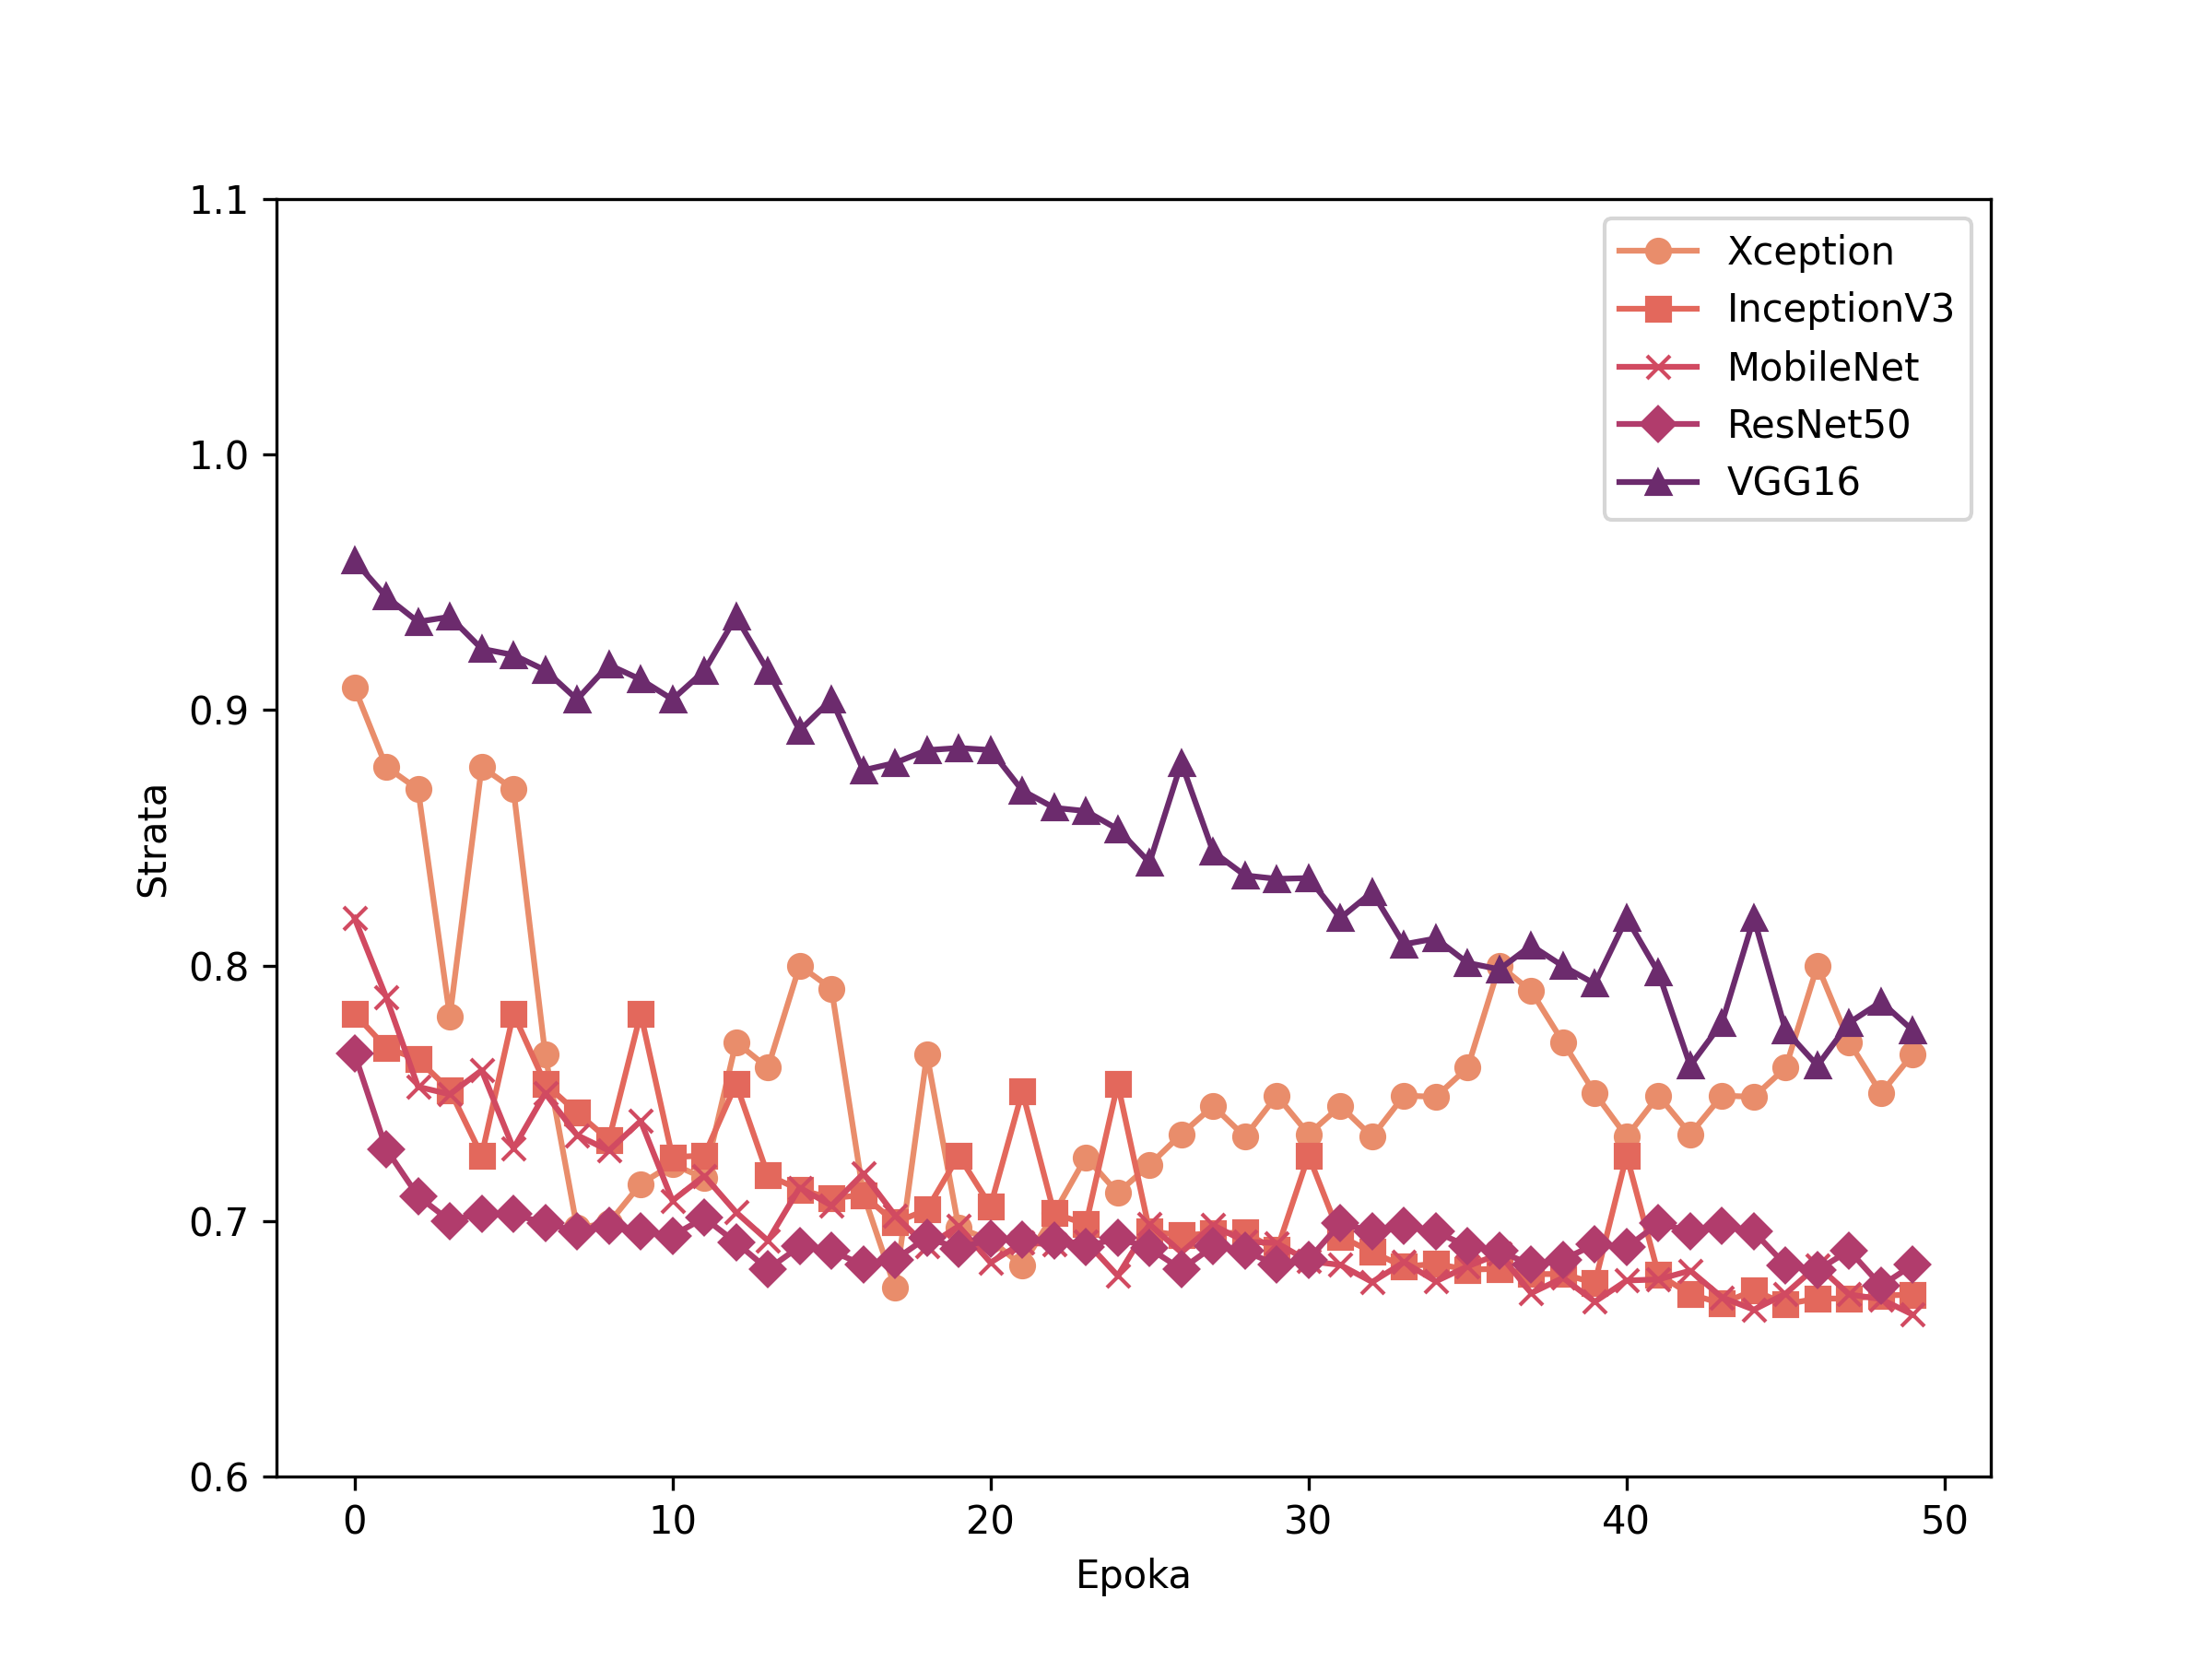
\includegraphics[width=\textwidth]{./img/results/i_loss}
        \caption{Krzywe funkcji straty na zbiorze walidacyjnym\@}
        \label{fig:i_loss}
    \end{subfigure}

    \caption{Porównanie krzywych uczenia dla różnych klasyfikatorów na zbiorze walidacyjnym (samogłoska /i/)}
    \label{fig:i_results}
\end{figure}

Na Rys.~\ref{fig:i_results} przedstawiono proces uczenia na zbiorze walidacyjnym dla samogłoski /i/.
Nie zaobserwowano oznak przeuczenia, a wykresy procesu uczenia są zbliżone do siebie.
Jedynie wartość funkcji straty jest znacznie wyższa w przypadku modelu VGG16 niż w pozostałych przypadkach.
Warto zauważyć, że proces uczenia wydaje się mniej stabilny w przypadku modeli Inception i Xception, co może wpływać na gorsze wyniki.

Mimo że żaden z tych modeli nie jest zalecany do wykorzystania w rzeczywistym środowisku, a wyniki dla innych samogłosek są wyższe, to nadal istnieje możliwość wykorzystania /i/ jako podstawy klasyfikacyjnej.
Konieczne jest jednak dokładniejsze zgłębienie tematu i specjalne dostosowanie metody.
%---------------------------------------------------------------------------

\section{Samogłoska /o/}
\label{sec:samogloska-o}

Wyniki uzyskane w przypadku samogłoski /o/ wykazują znaczne podobieństwo do tych uzyskanych w przypadku samogłoski /i/.
Dokładność klasyfikacji oscyluje między 61\% a 65\%, a funkcje straty są zbliżone (około 0,67).
Analizując wykresy procesu uczenia na Rys.~\ref{fig:o_results}, również można zaobserwować podobne zjawisko.

Na podstawie tych wyników nie da się wyróżnić optymalnego rozwiązania.
Konieczne jest pogłębienie analizy o więcej danych lub być może inne metody ekstrakcji cech.
Z pewnością istnieją markery, które pozwalają na odróżnienie osób chorych na PD od osób zdrowych na podstawie jednostki /i/, jednak nie są one tak wyraźne przy zastosowaniu wykorzystywanych w tym badaniu metod.

Podobieństwo wyników między samogłoskami /o/ i /i/ może sugerować, że te dwie samogłoski zawierają podobne cechy lub informacje diagnostyczne dla choroby Parkinsona.
Jednak warto zwrócić uwagę, że choć wyniki są zbliżone, to nie są one identyczne.
Istnieje subtelna różnica w dokładności klasyfikacji oraz wartościach funkcji straty, co może wynikać z różnic w akustyce lub wymowie tych dźwięków.

\begin{table}[ht]
\centering
\caption{Wyniki otrzymane dla samogłoski /o/}
\label{tab:wyniki-o}
\begin{tabular}{|l|c|c|c|c|c|}
\hline
\textbf{Model} &\textbf{VGG16} &\textbf{Resnet50} &\textbf{Xception} &\textbf{InceptionV3} &\textbf{MobileNetV2} \\ \hline
    Accuracy &0.653 &0.632 &0.653 &0.611 &0.611 \\ \hline
    Precision &0.654 &0.651 &0.651 &0.612 &0.624 \\ \hline
    Recall &0.649 &0.635 &0.649 &0.609 &0.606 \\ \hline
    F1-score &0.650 &0.633 &0.646 &0.601 &0.594 \\ \hline
    Loss &0.674 &0.679 &0.662 &0.679 &0.677\@ \\ \hline
\end{tabular}
\end{table}

\begin{figure}[ht]
    \centering
    \begin{subfigure}{0.49\textwidth}
        \centering
        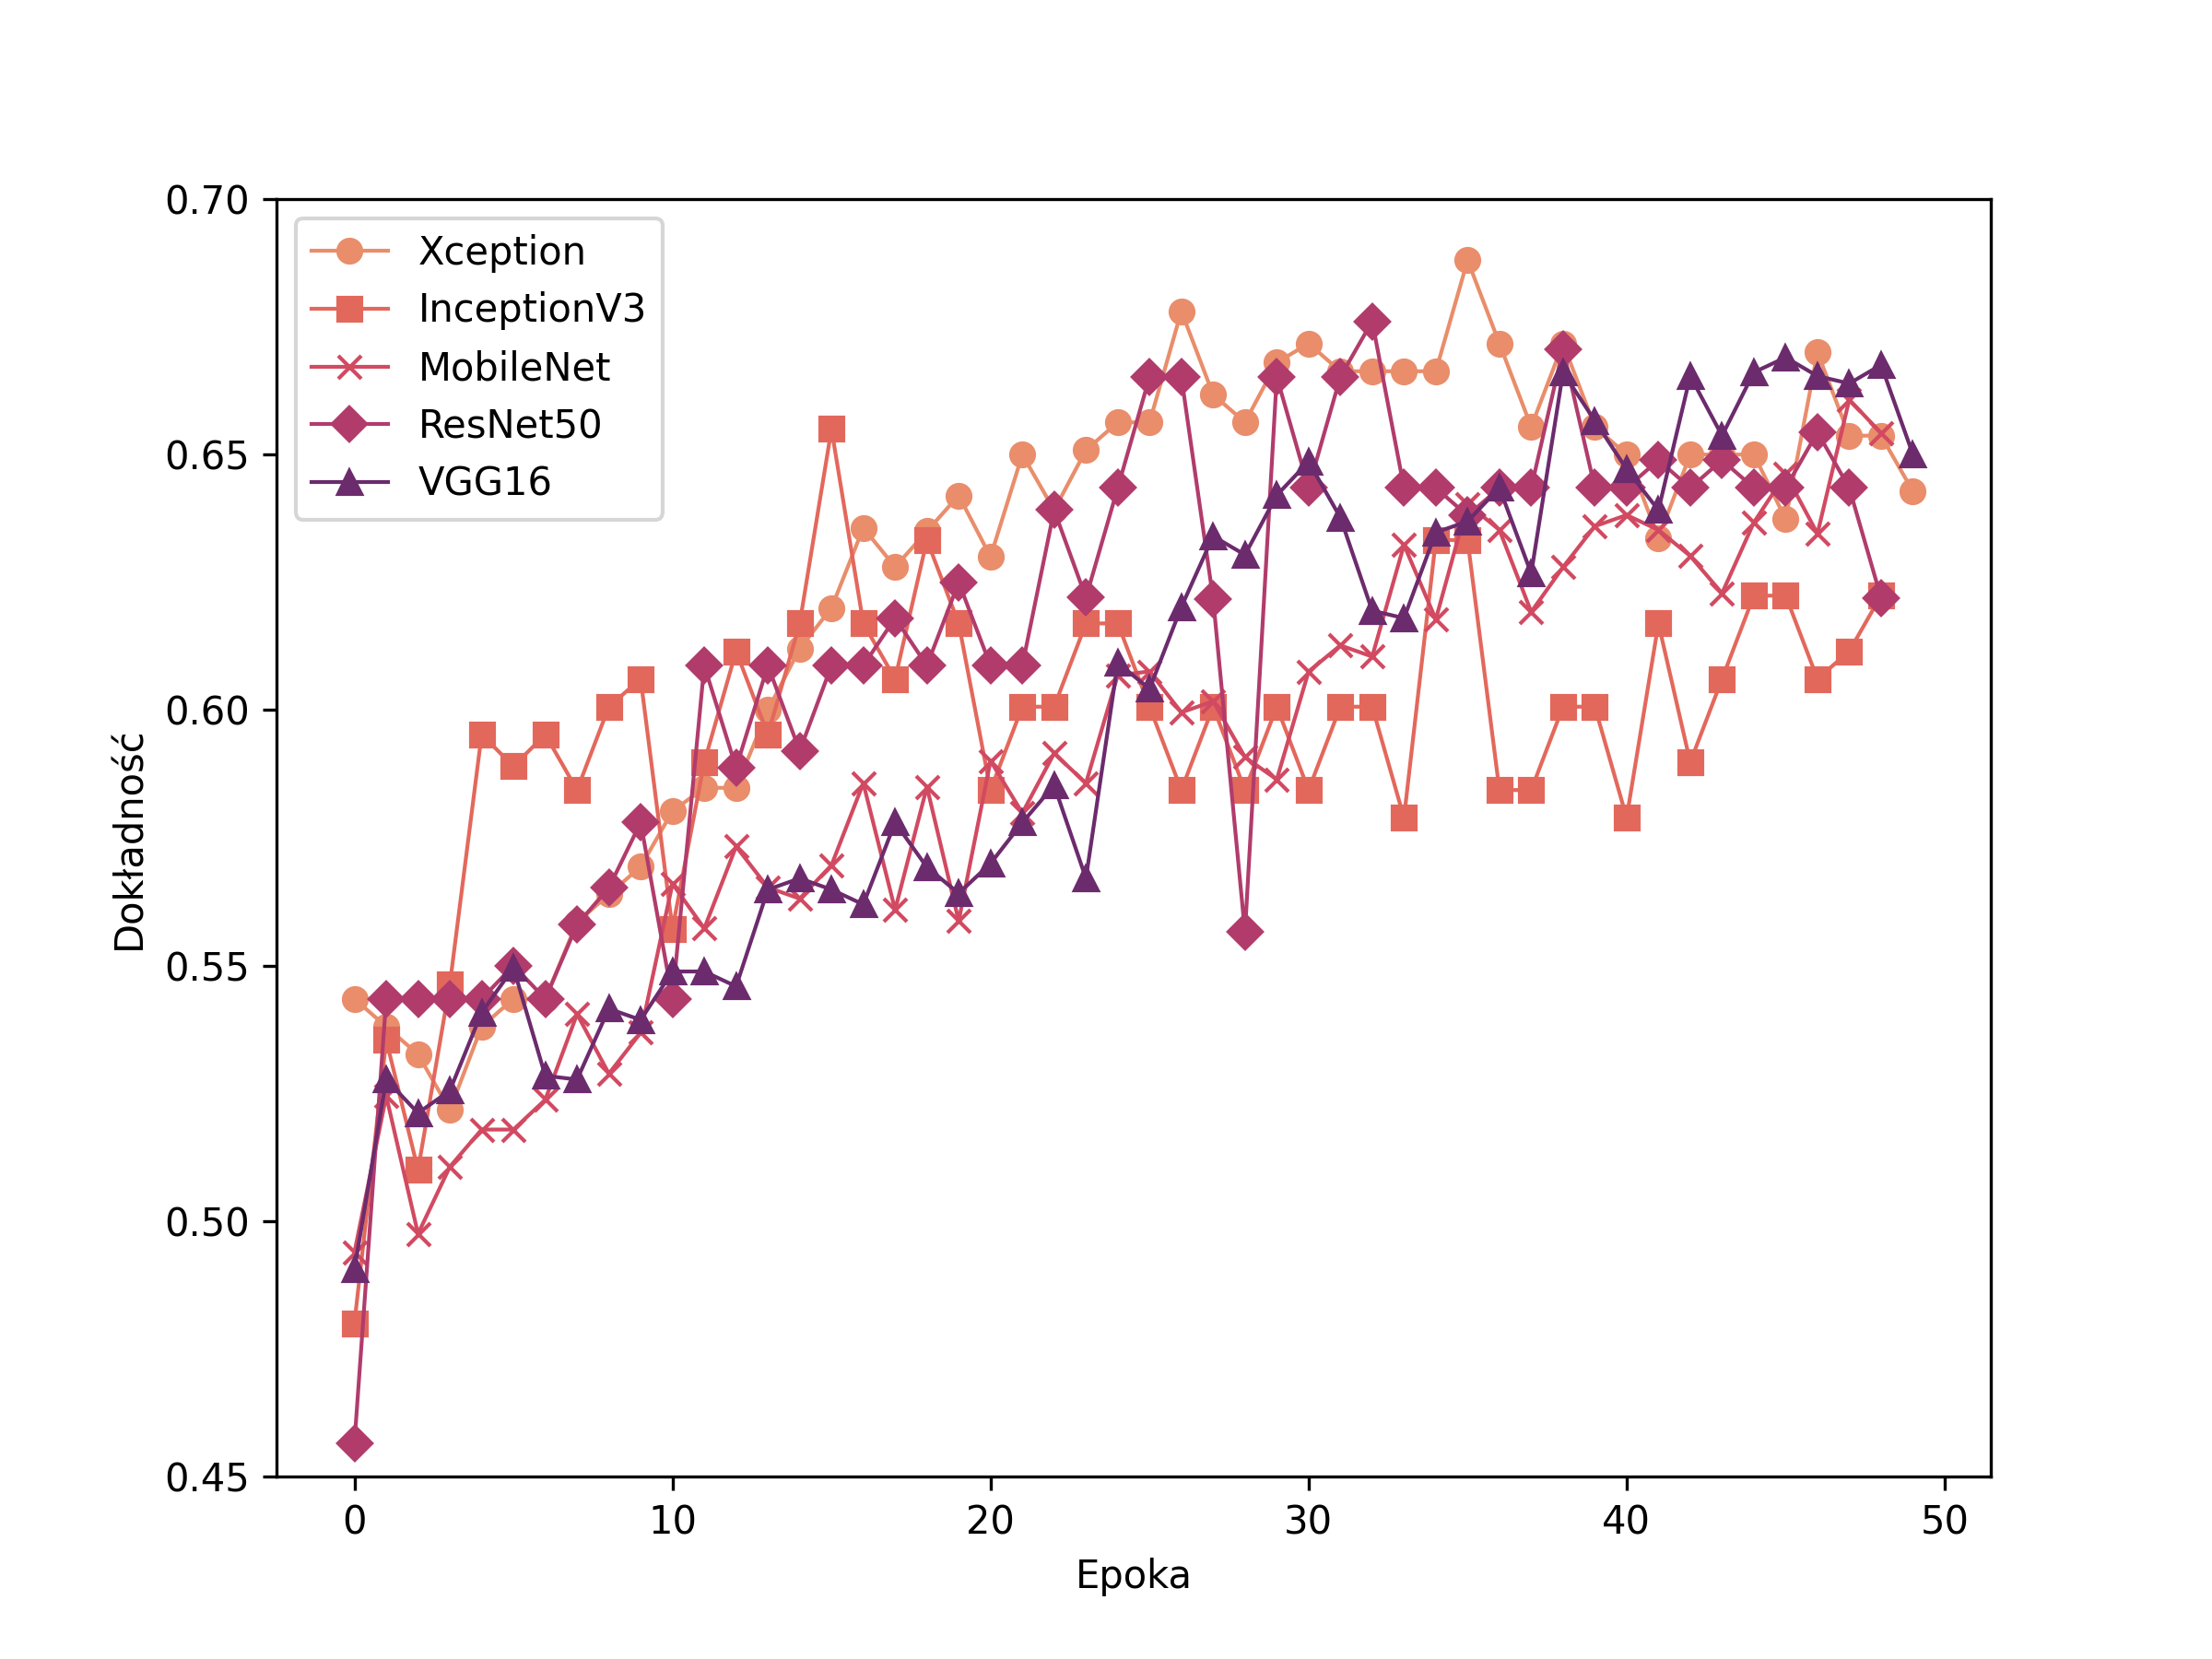
\includegraphics[width=\textwidth]{./img/results/o_acc}
        \caption{Krzywe dokładności na zbiorze walidacyjnym\@}
        \label{fig:o_acc}
    \end{subfigure}
    \begin{subfigure}{0.49\textwidth}
        \centering
        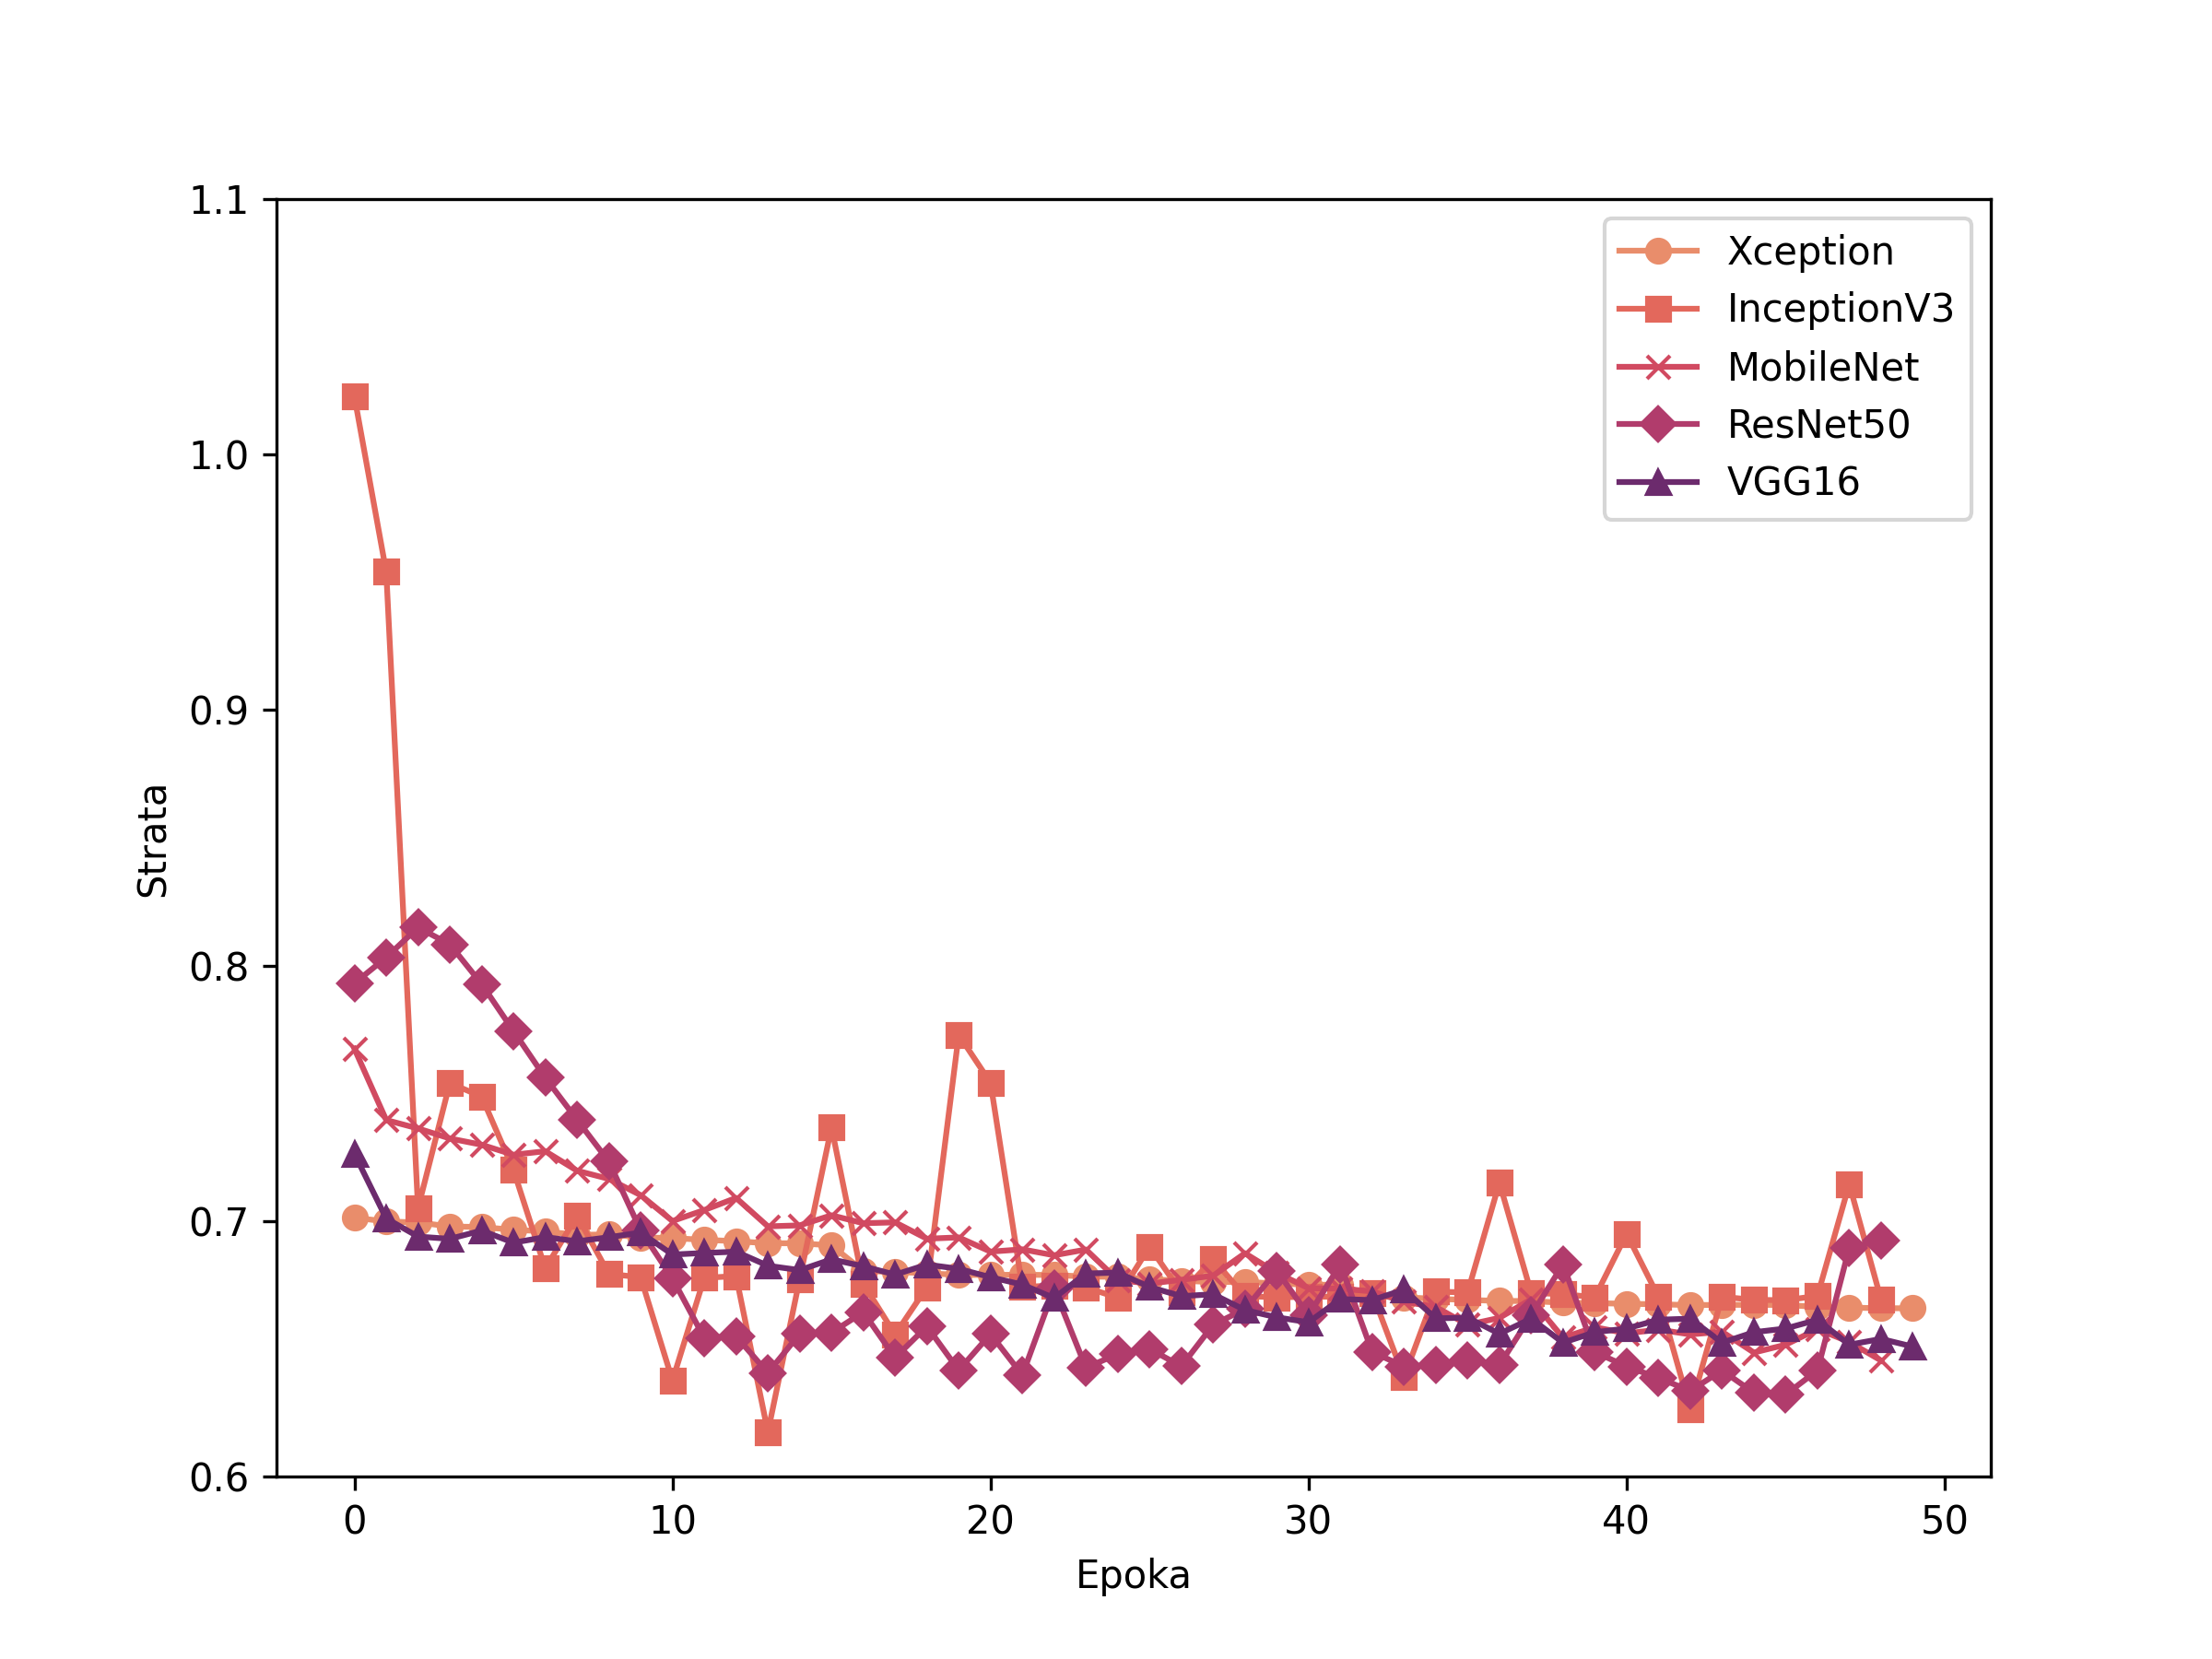
\includegraphics[width=\textwidth]{./img/results/o_loss}
        \caption{Krzywe funkcji straty na zbiorze walidacyjnym\@}
        \label{fig:o_loss}
    \end{subfigure}

    \caption{Porównanie krzywych uczenia dla różnych klasyfikatorów na zbiorze walidacyjnym (samogłoska /o/)}
    \label{fig:o_results}
\end{figure}

%---------------------------------------------------------------------------

\section{Samogłoska /u/}
\label{sec:samogloska-u}

W przypadku samogłoski /u/ obserwacje sugerują podobieństwo wyników do tych uzyskanych dla samogłoski /e/.
Tutaj również model VGG16 osiąga najlepsze wyniki, osiągając poziom skuteczności na poziomie 72\%.
Natomiast wyniki pozostałych modeli wahają się w zakresie od 64\% do 70\%.
Należy zwrócić uwagę na istotną różnicę w funkcji straty pomiędzy MobileNetV2 a pozostałymi modelami.
Wykazuje on znacząco wyższą wartość funkcji straty (0,750) w porównaniu do pozostałych modeli, które osiągają wartości w zakresie od 0,637 do 0,685.
Ta różnica może być istotna w kontekście oceny wydajności modeli.
Szczegółowe wartości przedstawia tabela~\ref{tab:wyniki-u}.


\begin{table}[ht]
\centering
\caption{Wyniki otrzymane dla samogłoski /u/}
\label{tab:wyniki-u}
\begin{tabular}{|l|c|c|c|c|c|}
\hline
\textbf{Model} &\textbf{VGG16} &\textbf{Resnet50} &\textbf{Xception} &\textbf{InceptionV3} &\textbf{MobileNetV2} \\ \hline
    Accuracy &0.724 &0.642 &0.663 &0.705 &0.642 \\ \hline
    Precision &0.730 &0.689 &0.682 &0.714 &0.686 \\ \hline
    Recall &0.715 &0.636 &0.657 &0.709 &0.635 \\ \hline
    F1-score &0.712 &0.615 &0.657 &0.708 &0.610 \\ \hline
    Loss &0.654 &0.685 &0.665 &0.637 &0.750 \\ \hline
\end{tabular}
\end{table}

\begin{figure}[ht]
    \centering
    \begin{subfigure}{0.49\textwidth}
        \centering
        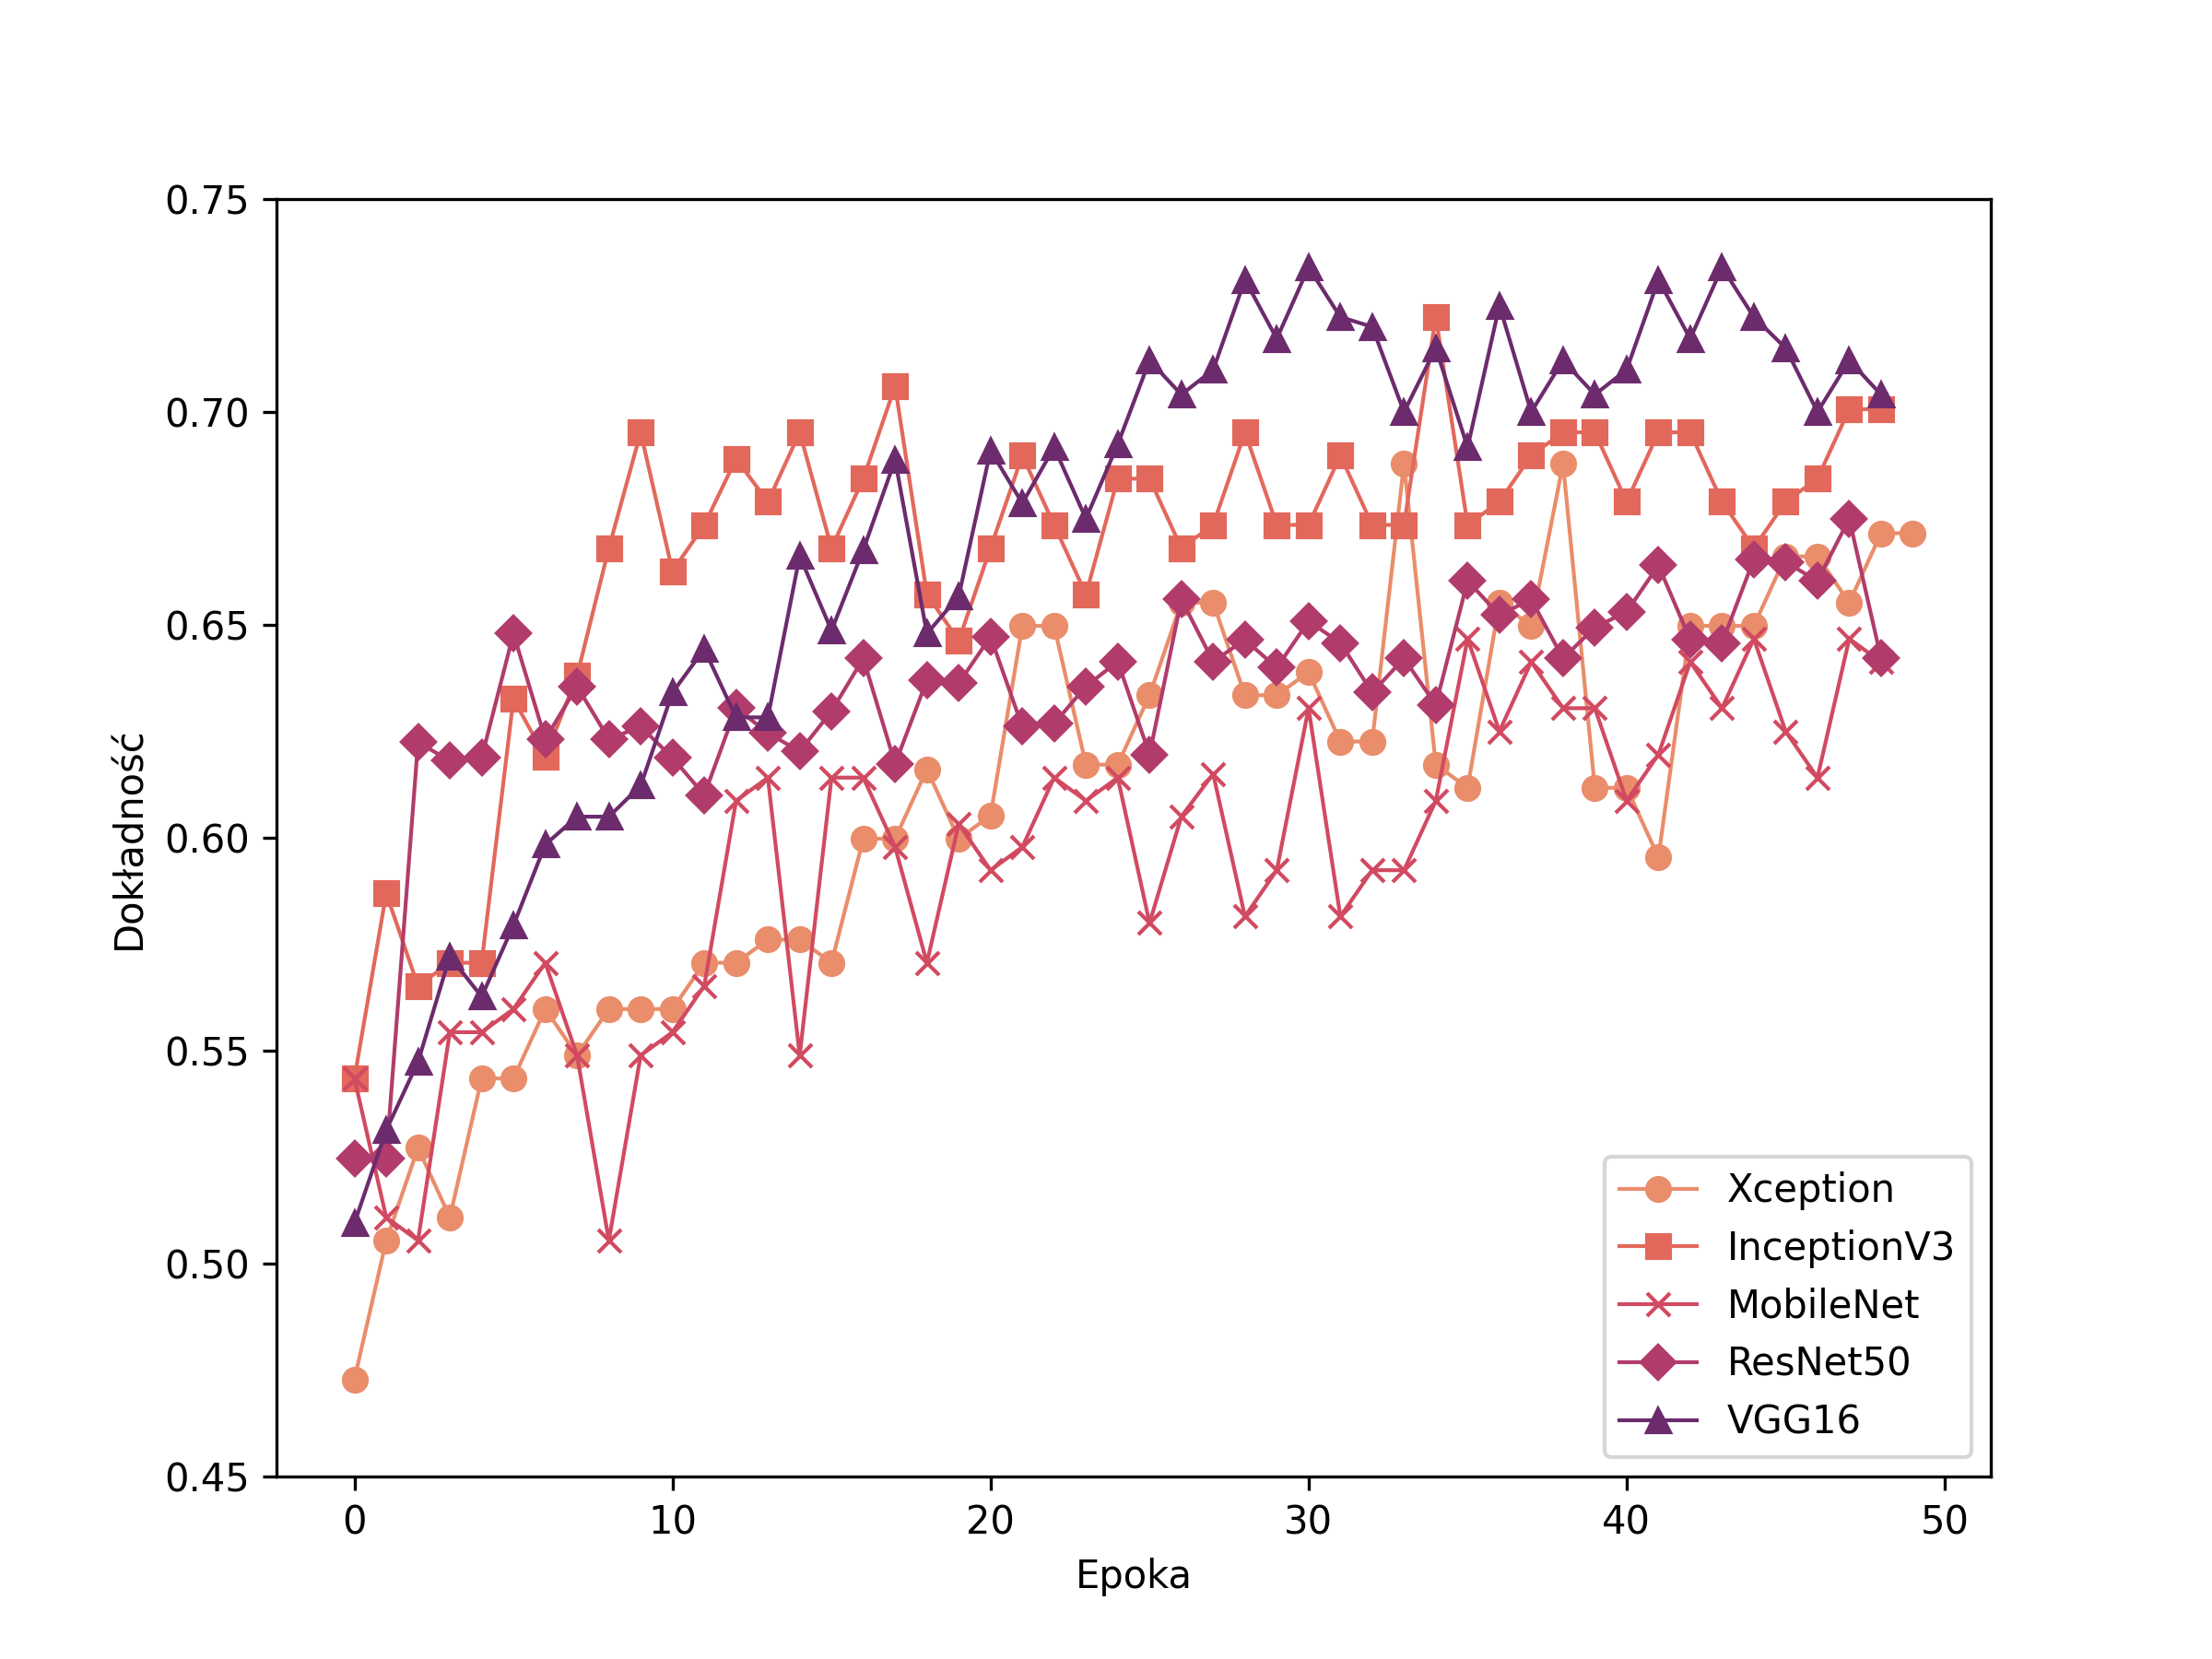
\includegraphics[width=\textwidth]{./img/results/u_acc}
        \caption{Krzywe dokładności na zbiorze walidacyjnym\@}
        \label{fig:u_acc}
    \end{subfigure}
    \begin{subfigure}{0.49\textwidth}
        \centering
        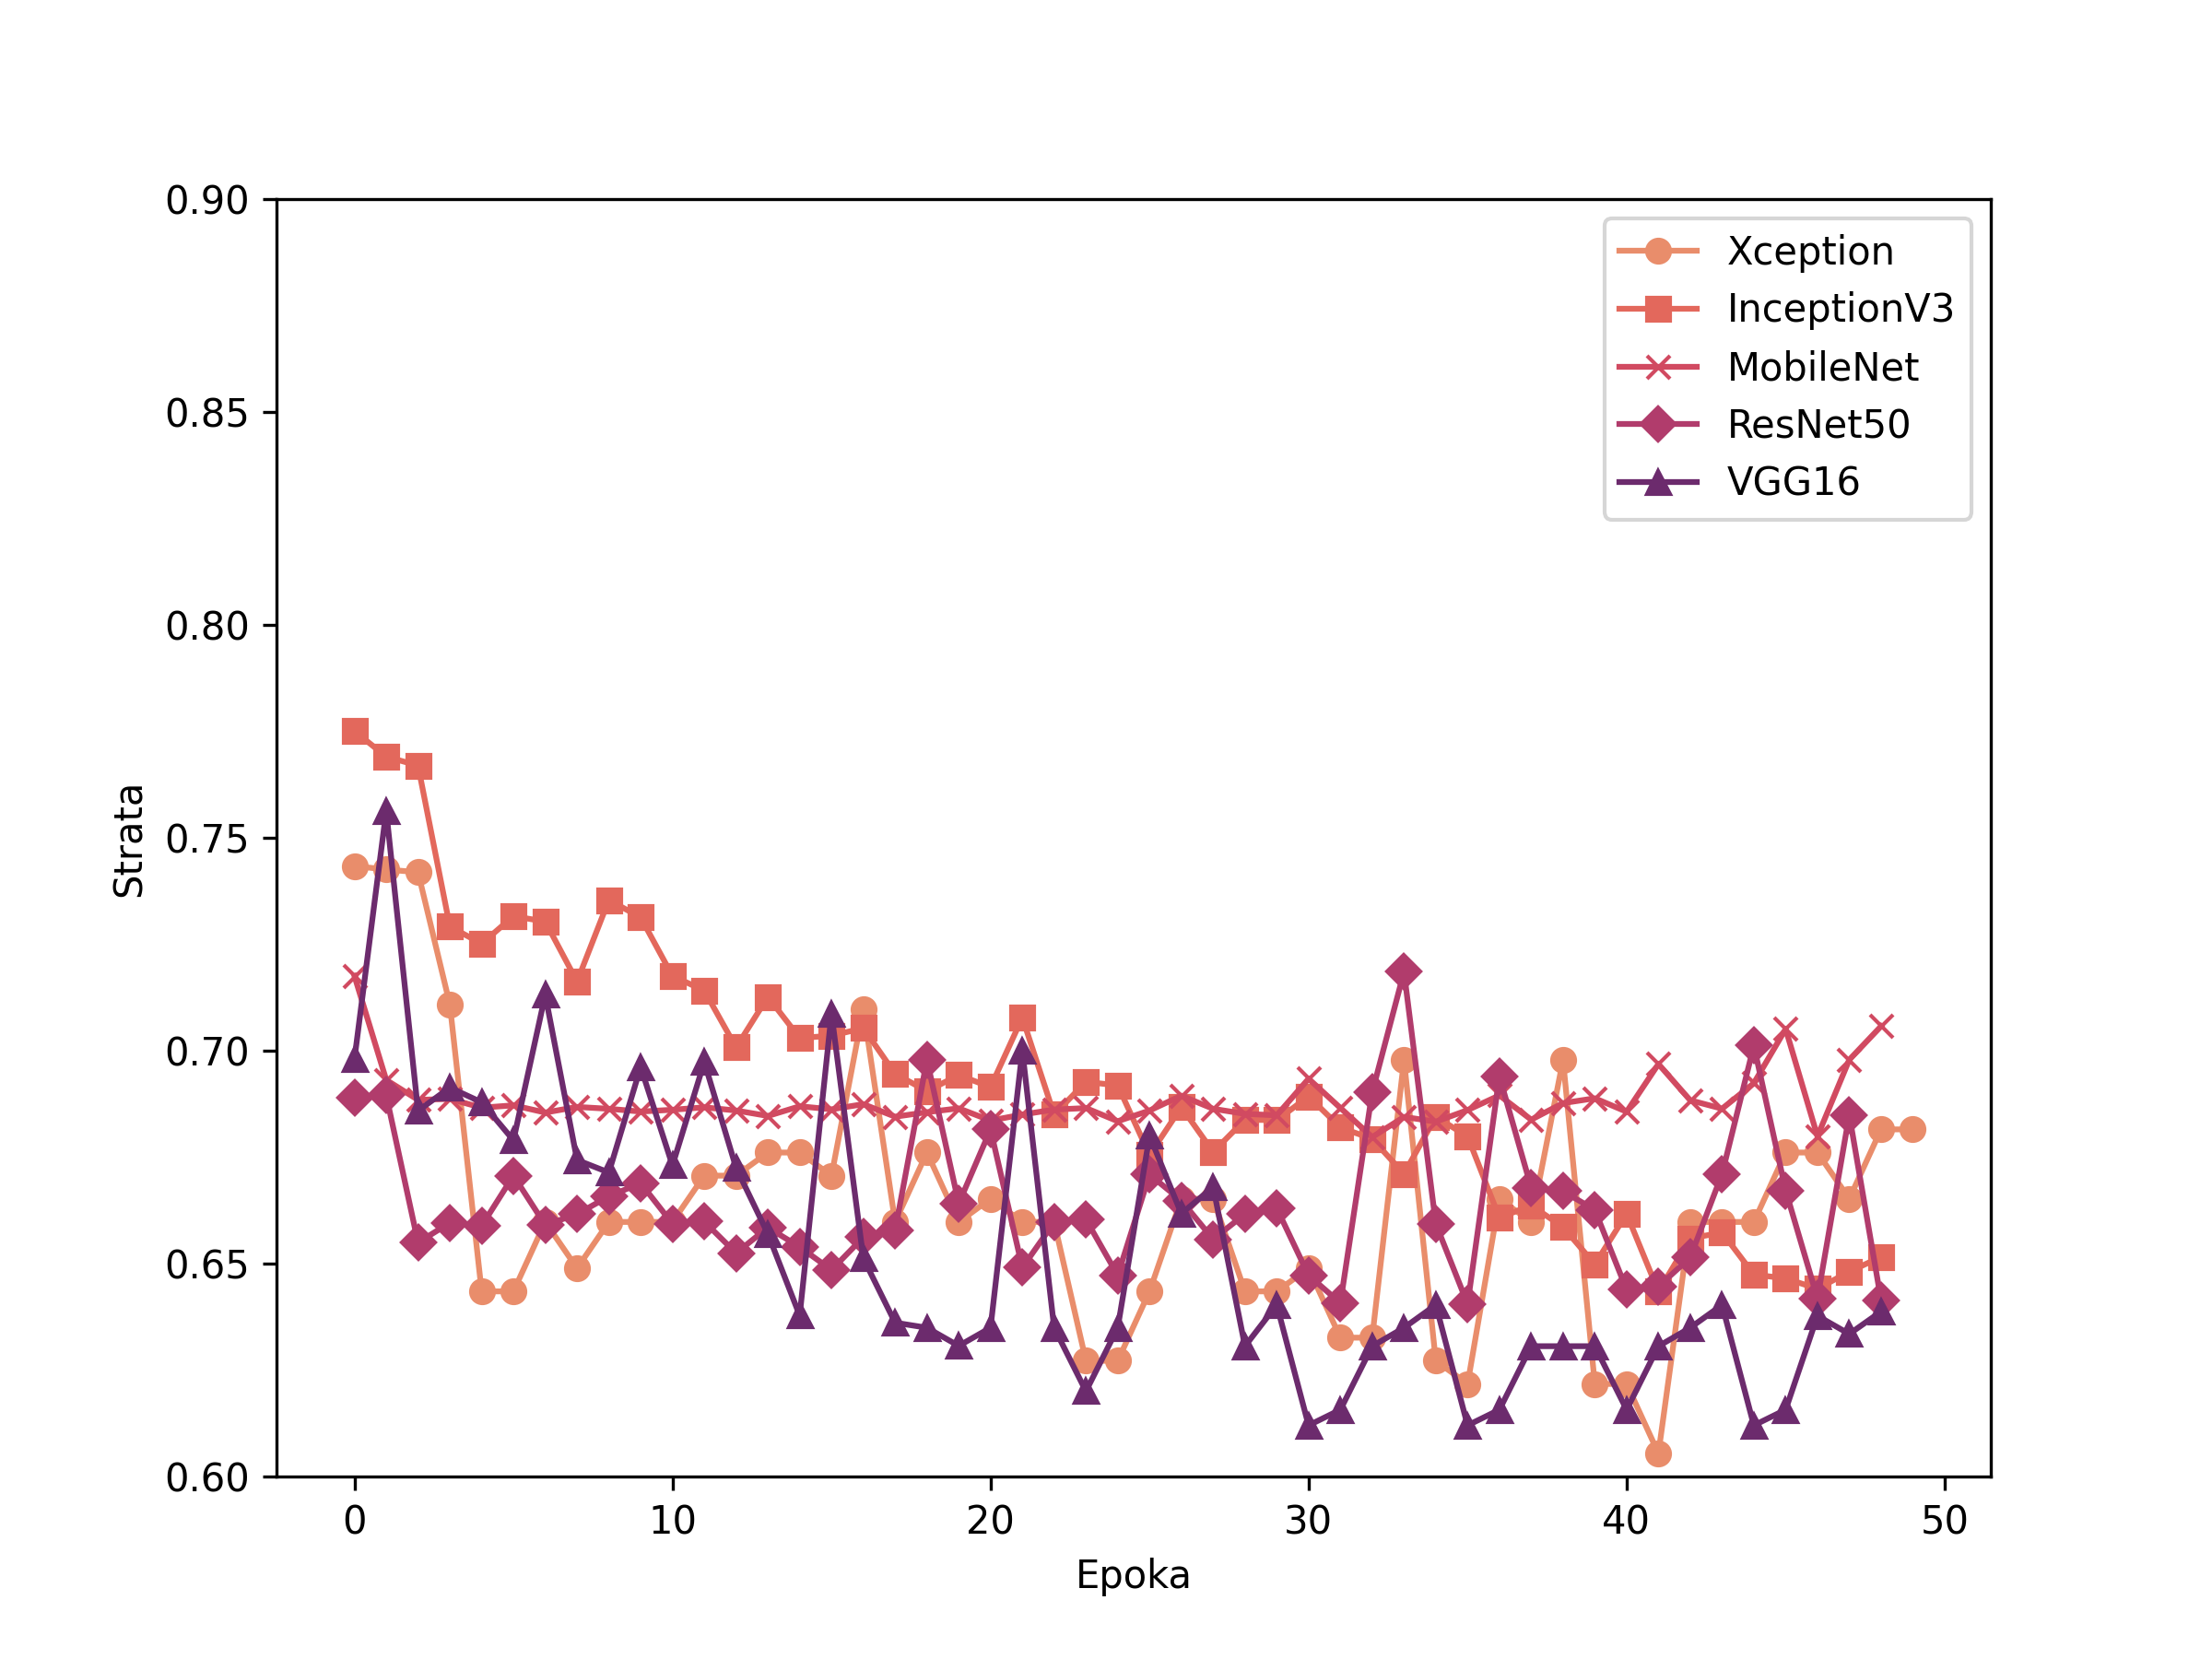
\includegraphics[width=\textwidth]{./img/results/u_loss}
        \caption{Krzywe funkcji straty na zbiorze walidacyjnym\@}
        \label{fig:u_loss}
    \end{subfigure}

    \caption{Porównanie krzywych uczenia dla różnych klasyfikatorów na zbiorze walidacyjnym (samogłoska /u/)}
    \label{fig:u_results}
\end{figure}

Analizując procesy uczenia testowanych modeli (Rys.~\ref{fig:u_results}), można zauważyć znaczne podobieństwo.
Warto zaznaczyć, że w przypadku MobileNetV2 funkcja straty pozostaje praktycznie stała przez cały proces uczenia, co nie jest pożądanym zjawiskiem.

%---------------------------------------------------------------------------
\section{Połączenie samogłosek /a/, /e/, /i/, /o/, /u/}
\label{sec:samogloski}


Zdecydowano się również zbadać skuteczność modeli trenowanych na zbiorze, który został stworzony przez połączenie wszystkich dotychczas badanych samogłosek.
Teoretycznie, taka praktyka mogła przyczynić się do poprawy wyników poprzez zwiększenie różnorodności zbioru danych.
Jednak nie przyniosła ona oczekiwanych efektów.
Może to wynikać z faktu, że rozszerzenie bazy nie zmieniło zestawu osób mówiących, a także możliwe, że markery choroby różnią się w zależności od wypowiadanej samogłoski.
Wyniki uzyskane w tym przypadku kształtują się w zakresie od 58\% do 63\%, a żadna z innych metryk nie wykazuje istotnych odchyleń od tego zakresu.
Warto również zwrócić uwagę na wartość funkcji straty, która utrzymuje się na poziomie około 0,7 z wyjątkiem modelu ResNet50, gdzie wartość ta znacząco odbiega i wynosi 0,970.
Cały raport został przedstawiony w tabeli~\ref{tab:wyniki-vowels}.

\begin{table}[ht]
\centering
\caption{Wyniki otrzymane dla połączenia samogłosek /a/, /e/, /i/, /o/ oraz /u/}
\label{tab:wyniki-vowels}
\begin{tabular}{|l|c|c|c|c|c|}
\hline
\textbf{Model} &\textbf{VGG16} &\textbf{Resnet50} &\textbf{Xception} &\textbf{InceptionV3} &\textbf{MobileNetV2} \\ \hline
    Accuracy &0.630 &0.577 &0.626 &0.615 &0.638 \\ \hline
    Precision &0.652 &0 578 &0.627 &0.621 &0.635 \\ \hline
    Recall &0.622 &0.575 &0.625 &0.611 &0.637 \\ \hline
    F1-score &0.598 &0.567 &0.631 &0.607 &0.639 \\ \hline
    Loss &0.692 &0.970 &0.654 &0.677 &0.645 \\ \hline
\end{tabular}
\end{table}

Znacznie odmienną wartość funkcji straty dla modelu ResNet50 można zobaczyć na Rys.~\ref{fig:vowels_results}.
Natomiast pozostałe modele wykazują bardzo niewielką zmienność w trakcie procesu uczenia, co przejawia się w niewielkim spadku tej wartości.
To zjawisko może sugerować, że ResNet50 doświadczało pewnych trudności lub przeszkód w procesie uczenia, które nie występowały w przypadku innych modeli.


\begin{figure}[ht]
    \centering
    \begin{subfigure}{0.49\textwidth}
        \centering
        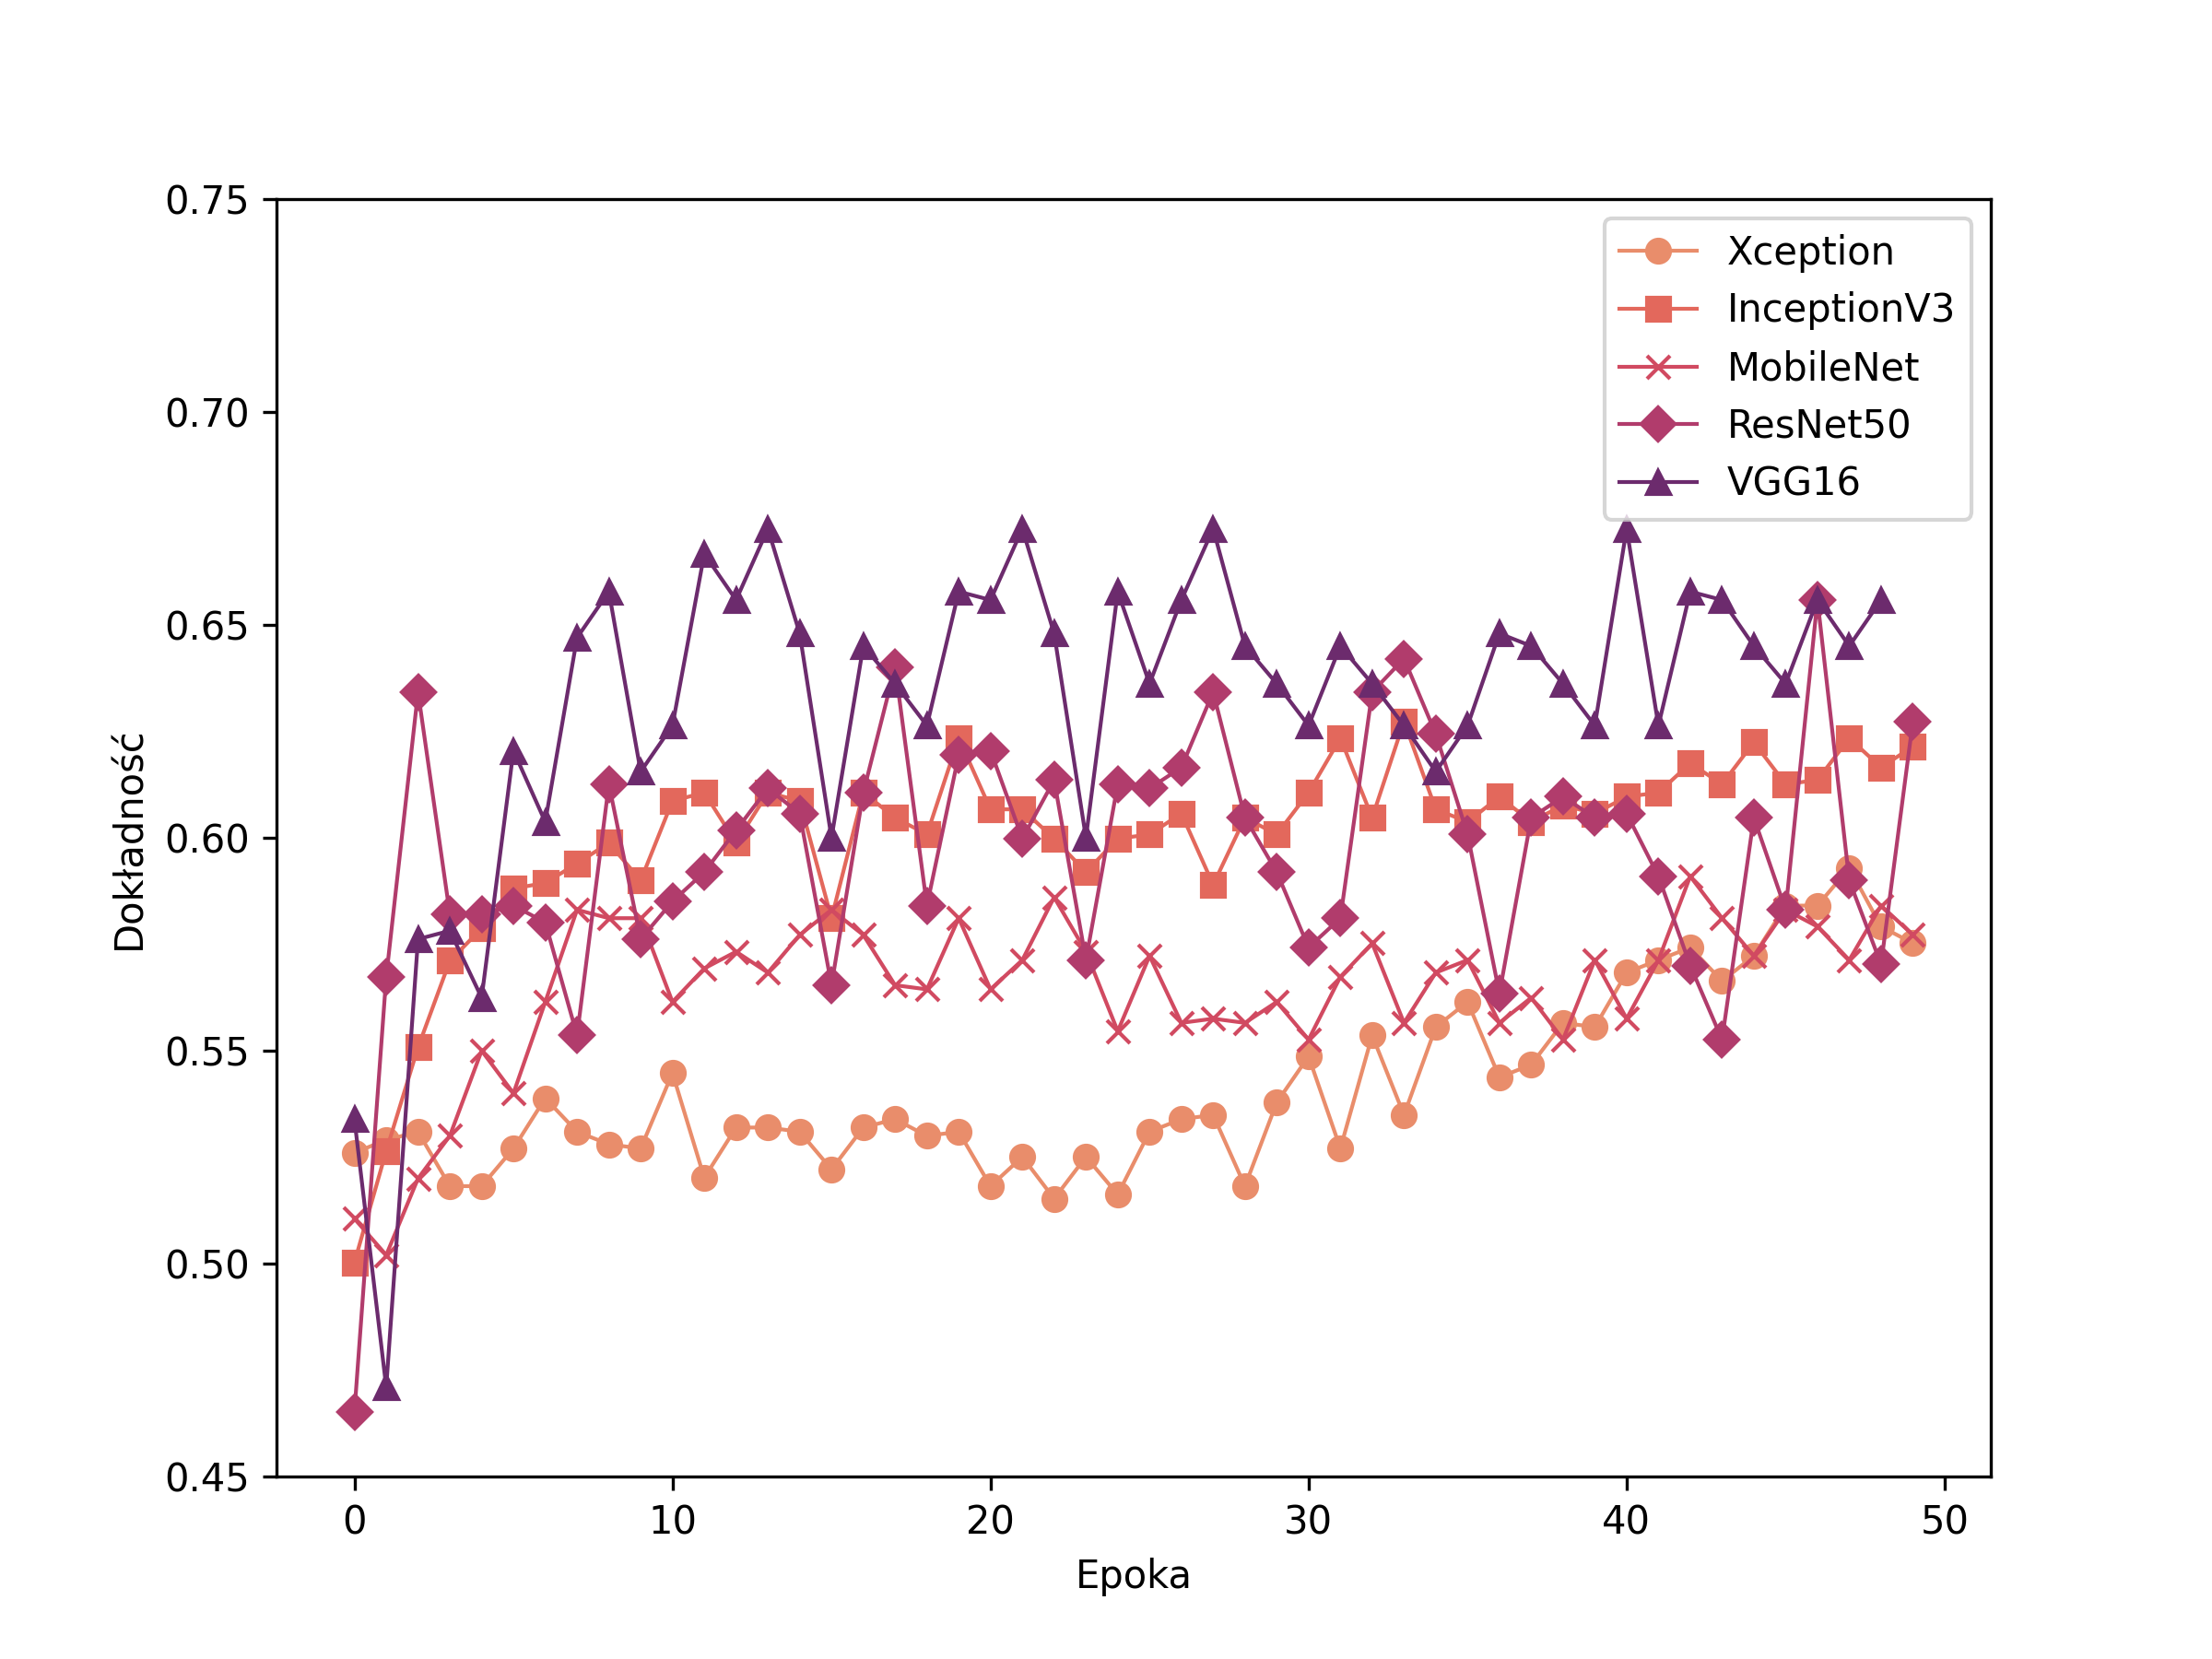
\includegraphics[width=\textwidth]{./img/results/all_acc}
        \caption{Krzywe dokładności na zbiorze walidacyjnym\@}
        \label{fig:vowels_acc}
    \end{subfigure}
    \begin{subfigure}{0.49\textwidth}
        \centering
        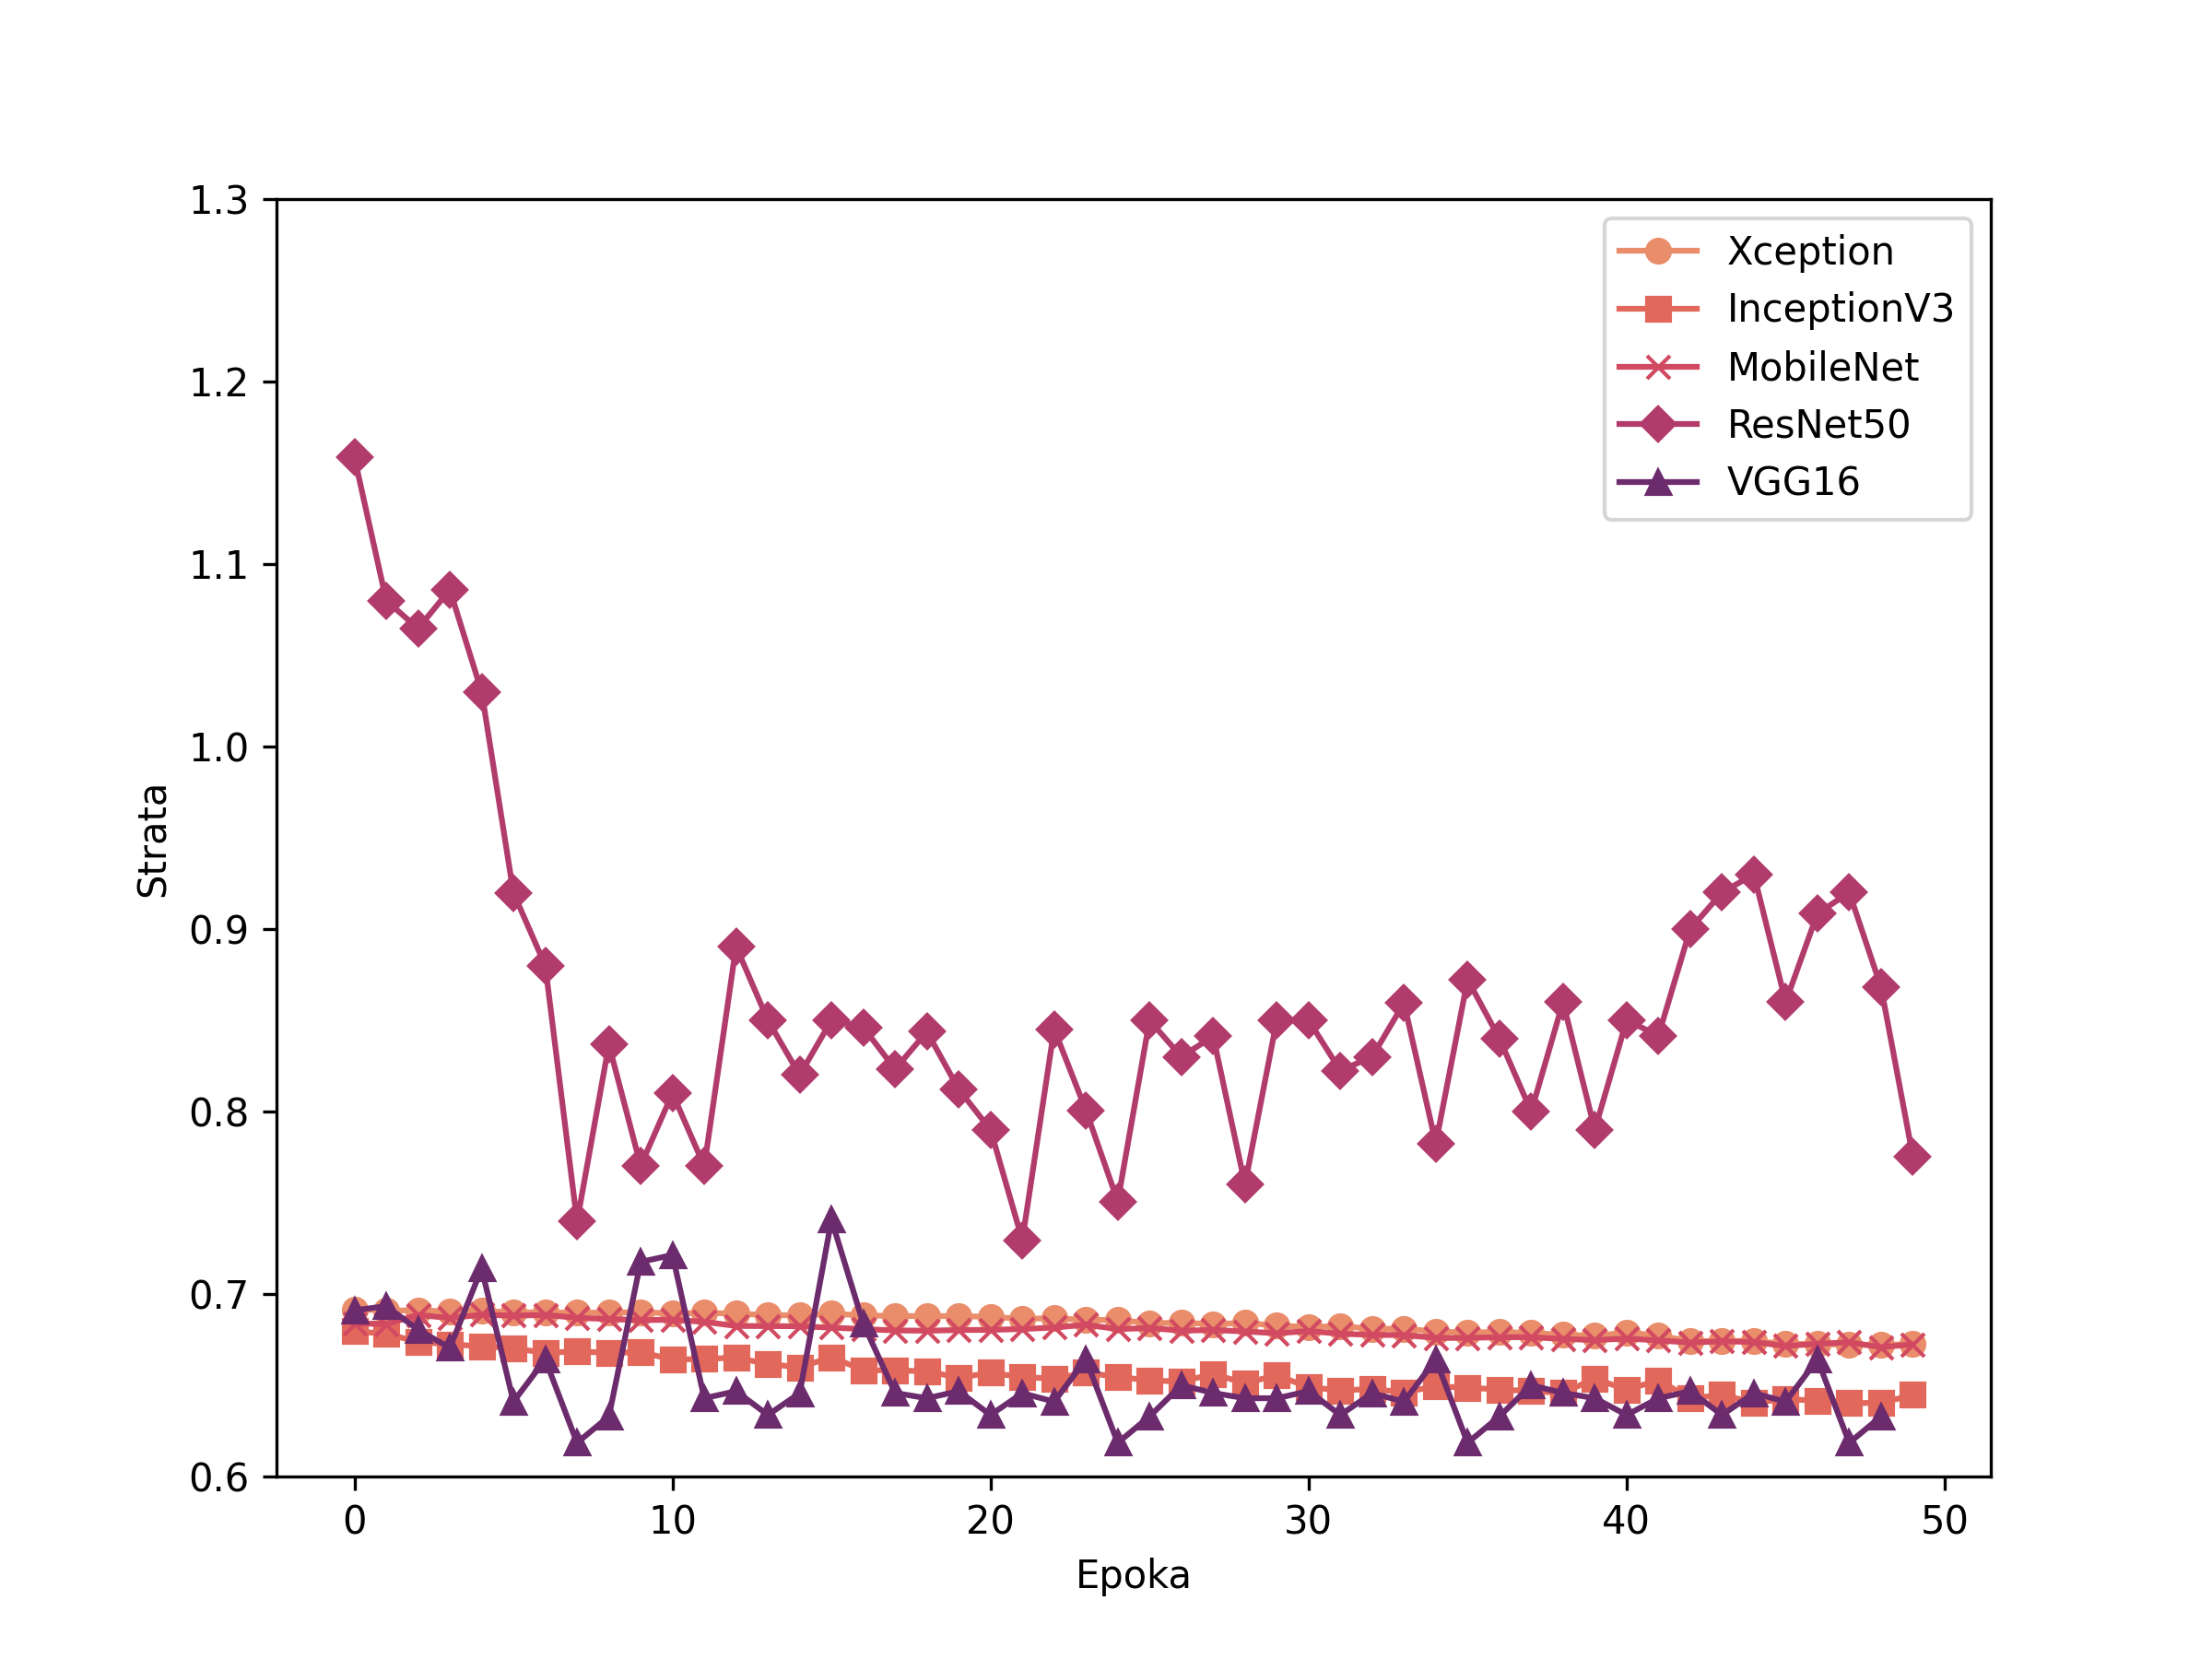
\includegraphics[width=\textwidth]{./img/results/all_loss}
        \caption{Krzywe funkcji straty na zbiorze walidacyjnym\@}
        \label{fig:vowels_loss}
    \end{subfigure}

    \caption{Porównanie krzywych uczenia dla różnych klasyfikatorów na zbiorze walidacyjnym (połączenie samogłosek /a/, /e/, /i/, /o/ oraz /u/)}
    \label{fig:vowels_results}
\end{figure}

%---------------------------------------------------------------------------

\section{Zbiorcze podsumowanie wyników}
\label{sec:podsumowanie-wynikow}

Na podstawie przedstawionych do tej pory wyników, zebrano najlepsze z nich w Tab.~\ref{tab:wyniki-podsumowanie}, aby ułatwić ich porównanie.
Najlepsze osiągnięcia zostały zarejestrowane dla samogłosek /a/, /e/ oraz /u/, gdzie dokładność przekroczyła 70\%.
W przypadku /i/ oraz /o/, a także połączenia wszystkich samogłosek, wyniki były znacznie niższe i utrzymywały się na poziomie około 65\%.
Pozostałe metryki są zbliżone, co wskazuje na podobną jakość rozpoznawania każdej z klas.
Oznacza to, że prawdopodobieństwo popełnienia błędu I jak i II rodzaju są bardzo podobne.
Warto zaznaczyć, że w analizowanym problemie badawczym szczególnie istotna jest minimalizacja błędu II rodzaju.

Jeśli chodzi o architektury, to najczęściej najlepiej radził sobie model VGG16, osiągając najwyższą skuteczność w przypadku 4 z 6 analizowanych przypadków.
Obiecująco wypadły także modele Xception i MobileNetV2 w przypadku samogłosek /i/ oraz /o/.

\begin{table}[ht]
\centering
\caption{Najlepsze z otrzymanych wyników dla poszczególnych wariantów badanych samogłosek\@}
\label{tab:wyniki-podsumowanie}
\begin{tabular}{|l|c|c|c|c|c|c|}
\hline
\textbf{Samogłoska} &\textbf{/a/} &\textbf{/e/} &\textbf{/i/} &\textbf{/o/} &\textbf{/u/}  &\textbf{wszystkie samogłoski}\\ \hline
    Model  &VGG16 &VGG16 &Xception &VGG16 &VGG16 &MobileNetV2 \\ \hline
    Accuracy  &0.751 &0.733 &0.641 &0.653 &0.724 &0.638 \\ \hline
    Precision  &0.752 &0.729 &0.638 &0.654 &0.730 &0.635 \\ \hline
    Recall  &0.751 &0.733 &0.642 &0.649 &0.715 &0.637 \\ \hline
    F1-score &0.749 &0.75 &0.643 &0.650 &0.712 &0.639 \\ \hline
    Loss &0.645 &0.582 &0.705 &0.674 &0.654 &0.645 \\ \hline
\end{tabular}
\end{table}

Warto zaznaczyć, że funkcja straty utrzymywała się na stosunkowo wysokim poziomie we wszystkich analizowanych przypadkach, co może sugerować pewne trudności lub wyzwania w procesie uczenia.
Istnieje możliwość, że optymalizacja modeli mogłaby być bardziej precyzyjna, aby osiągnąć niższą wartość funkcji straty i poprawić skuteczność klasyfikacji.
Dalsza analiza i eksperymenty mogą być potrzebne w celu doskonalenia wydajności modeli.